\documentclass[twoside]{book}

% Packages required by doxygen
\usepackage{fixltx2e}
\usepackage{calc}
\usepackage{doxygen}
\usepackage{graphicx}
\usepackage[utf8]{inputenc}
\usepackage{makeidx}
\usepackage{multicol}
\usepackage{multirow}
\PassOptionsToPackage{warn}{textcomp}
\usepackage{textcomp}
\usepackage[nointegrals]{wasysym}
\usepackage[table]{xcolor}
\usepackage{ifpdf,ifxetex}

% Font selection
\usepackage[T1]{fontenc}
\usepackage[scaled=.90]{helvet}
\usepackage{courier}
\usepackage{amssymb}
\usepackage{sectsty}
\renewcommand{\familydefault}{\sfdefault}
\allsectionsfont{%
  \fontseries{bc}\selectfont%
  \color{darkgray}%
}
\renewcommand{\DoxyLabelFont}{%
  \fontseries{bc}\selectfont%
  \color{darkgray}%
}
\newcommand{\+}{\discretionary{\mbox{\scriptsize$\hookleftarrow$}}{}{}}

% Page & text layout
\usepackage{geometry}
\geometry{%
  a4paper,%
  top=2.5cm,%
  bottom=2.5cm,%
  left=2.5cm,%
  right=2.5cm%
}
\tolerance=750
\hfuzz=15pt
\hbadness=750
\setlength{\emergencystretch}{15pt}
\setlength{\parindent}{0cm}
\setlength{\parskip}{3ex plus 2ex minus 2ex}
\makeatletter
\renewcommand{\paragraph}{%
  \@startsection{paragraph}{4}{0ex}{-1.0ex}{1.0ex}{%
    \normalfont\normalsize\bfseries\SS@parafont%
  }%
}
\renewcommand{\subparagraph}{%
  \@startsection{subparagraph}{5}{0ex}{-1.0ex}{1.0ex}{%
    \normalfont\normalsize\bfseries\SS@subparafont%
  }%
}
\makeatother

% Headers & footers
\usepackage{fancyhdr}
\pagestyle{fancyplain}
\fancyhead[LE]{\fancyplain{}{\bfseries\thepage}}
\fancyhead[CE]{\fancyplain{}{}}
\fancyhead[RE]{\fancyplain{}{\bfseries\leftmark}}
\fancyhead[LO]{\fancyplain{}{\bfseries\rightmark}}
\fancyhead[CO]{\fancyplain{}{}}
\fancyhead[RO]{\fancyplain{}{\bfseries\thepage}}
\fancyfoot[LE]{\fancyplain{}{}}
\fancyfoot[CE]{\fancyplain{}{}}
\fancyfoot[RE]{\fancyplain{}{\bfseries\scriptsize Generated by Doxygen }}
\fancyfoot[LO]{\fancyplain{}{\bfseries\scriptsize Generated by Doxygen }}
\fancyfoot[CO]{\fancyplain{}{}}
\fancyfoot[RO]{\fancyplain{}{}}
\renewcommand{\footrulewidth}{0.4pt}
\renewcommand{\chaptermark}[1]{%
  \markboth{#1}{}%
}
\renewcommand{\sectionmark}[1]{%
  \markright{\thesection\ #1}%
}

% Indices & bibliography
\usepackage{natbib}
\usepackage[titles]{tocloft}
\setcounter{tocdepth}{3}
\setcounter{secnumdepth}{5}
\makeindex

% Hyperlinks (required, but should be loaded last)
\ifpdf
  \usepackage[pdftex,pagebackref=true]{hyperref}
\else
  \ifxetex
    \usepackage[pagebackref=true]{hyperref}
  \else
    \usepackage[ps2pdf,pagebackref=true]{hyperref}
  \fi
\fi
\ifpdf
  \DeclareUnicodeCharacter{207B}{${}^{-}$}% Superscript minus
  \DeclareUnicodeCharacter{C2B2}{${}^{2}$}% Superscript two
  \DeclareUnicodeCharacter{C2B3}{${}^{3}$}% Superscript three
\else
  \catcode`\⁻=13% Superscript minus
  \def⁻{${}^{-}$}
  \catcode`\²=13% Superscript two
  \def²{${}^{2}$}
  \catcode`\³=13% Superscript three
  \def³{${}^{3}$}
\fi

\hypersetup{%
  colorlinks=true,%
  linkcolor=blue,%
  citecolor=blue,%
  unicode%
}

% Custom commands
\newcommand{\clearemptydoublepage}{%
  \newpage{\pagestyle{empty}\cleardoublepage}%
}

\usepackage{caption}
\captionsetup{labelsep=space,justification=centering,font={bf},singlelinecheck=off,skip=4pt,position=top}

\renewcommand{\numberline}[1]{#1~}
%===== C O N T E N T S =====

\begin{document}

% Titlepage & ToC
\hypersetup{pageanchor=false,
             bookmarksnumbered=true,
             pdfencoding=unicode
            }
\pagenumbering{alph}
\begin{titlepage}
\vspace*{7cm}
\begin{center}%
{\Large My Project }\\
\vspace*{1cm}
{\large Generated by Doxygen 1.8.15}\\
\end{center}
\end{titlepage}
\clearemptydoublepage
\pagenumbering{roman}
\tableofcontents
\clearemptydoublepage
\pagenumbering{arabic}
\hypersetup{pageanchor=true}

%--- Begin generated contents ---
\chapter{Namespace Index}
\section{Namespace List}
Here is a list of all documented namespaces with brief descriptions\+:\begin{DoxyCompactList}
\item\contentsline{section}{\mbox{\hyperlink{namespacecpyp}{cpyp}} }{\pageref{namespacecpyp}}{}
\end{DoxyCompactList}

\chapter{Hierarchical Index}
\section{Class Hierarchy}
This inheritance list is sorted roughly, but not completely, alphabetically\+:\begin{DoxyCompactList}
\item \contentsline{section}{cpyp\+:\+:bintied\+\_\+parameter\+\_\+resampler$<$ C\+RP $>$}{\pageref{structcpyp_1_1bintied__parameter__resampler}}{}
\item \contentsline{section}{cpyp\+:\+:Sparse\+Vector$<$ T, L\+O\+C\+A\+L\+\_\+\+M\+AX $>$\+:\+:const\+\_\+iterator}{\pageref{structcpyp_1_1_sparse_vector_1_1const__iterator}}{}
\item \contentsline{section}{cpyp\+:\+:crp$<$ Dish, Dish\+Hash $>$}{\pageref{classcpyp_1_1crp}}{}
\item \contentsline{section}{cpyp\+:\+:crp\+\_\+histogram}{\pageref{structcpyp_1_1crp__histogram}}{}
\item \contentsline{section}{cpyp\+:\+:crp\+\_\+table\+\_\+manager$<$ Num\+Floors $>$}{\pageref{structcpyp_1_1crp__table__manager}}{}
\item \contentsline{section}{cpyp\+:\+:Dict}{\pageref{classcpyp_1_1_dict}}{}
\item \contentsline{section}{cpyp\+:\+:gamma\+\_\+poisson$<$ F $>$}{\pageref{structcpyp_1_1gamma__poisson}}{}
\item \contentsline{section}{cpyp\+:\+:Sparse\+Vector$<$ T, L\+O\+C\+A\+L\+\_\+\+M\+AX $>$\+:\+:iterator}{\pageref{structcpyp_1_1_sparse_vector_1_1iterator}}{}
\item \contentsline{section}{Log\+Val$<$ T $>$}{\pageref{class_log_val}}{}
\item \contentsline{section}{cpyp\+:\+:M$<$ F $>$}{\pageref{structcpyp_1_1_m}}{}
\item \contentsline{section}{cpyp\+:\+:mf\+\_\+crp$<$ Num\+Floors, Dish, Dish\+Hash $>$}{\pageref{classcpyp_1_1mf__crp}}{}
\item mt19937\begin{DoxyCompactList}
\item \contentsline{section}{cpyp\+:\+:MT19937}{\pageref{structcpyp_1_1_m_t19937}}{}
\end{DoxyCompactList}
\item \contentsline{section}{cpyp\+:\+:multinomial\+\_\+distribution$<$ F $>$}{\pageref{structcpyp_1_1multinomial__distribution}}{}
\item \contentsline{section}{cpyp\+:\+:Pair\+IntT$<$ T $>$}{\pageref{structcpyp_1_1_pair_int_t}}{}
\item \contentsline{section}{cpyp\+:\+:Pair\+IntT$<$ unsigned $>$}{\pageref{structcpyp_1_1_pair_int_t}}{}
\item \contentsline{section}{cpyp\+:\+:P\+Y\+P\+LM$<$ N $>$}{\pageref{structcpyp_1_1_p_y_p_l_m}}{}
\item \contentsline{section}{cpyp\+:\+:slice\+\_\+sampler\+\_\+rfc\+\_\+type$<$ F, Fn, U $>$}{\pageref{structcpyp_1_1slice__sampler__rfc__type}}{}
\item \contentsline{section}{cpyp\+:\+:Sparse\+Vector$<$ T, L\+O\+C\+A\+L\+\_\+\+M\+AX $>$}{\pageref{classcpyp_1_1_sparse_vector}}{}
\item \contentsline{section}{cpyp\+:\+:Sparse\+Vector$<$ unsigned $>$}{\pageref{classcpyp_1_1_sparse_vector}}{}
\item \contentsline{section}{cpyp\+:\+:S\+P\+Y\+P\+LM$<$ N $>$}{\pageref{classcpyp_1_1_s_p_y_p_l_m}}{}
\item \contentsline{section}{cpyp\+:\+:tied\+\_\+parameter\+\_\+resampler$<$ C\+RP $>$}{\pageref{structcpyp_1_1tied__parameter__resampler}}{}
\item \contentsline{section}{cpyp\+:\+:tied\+\_\+parameter\+\_\+resampler$<$ cpyp\+:\+:crp$<$ unsigned $>$ $>$}{\pageref{structcpyp_1_1tied__parameter__resampler}}{}
\item \contentsline{section}{cpyp\+:\+:Uniform\+Vocabulary}{\pageref{structcpyp_1_1_uniform_vocabulary}}{}
\begin{DoxyCompactList}
\item \contentsline{section}{cpyp\+:\+:P\+Y\+P\+LM$<$ 0 $>$}{\pageref{structcpyp_1_1_p_y_p_l_m_3_010_01_4}}{}
\end{DoxyCompactList}
\item \contentsline{section}{uvector\+\_\+hash}{\pageref{structuvector__hash}}{}
\end{DoxyCompactList}

\chapter{Class Index}
\section{Class List}
Here are the classes, structs, unions and interfaces with brief descriptions\+:\begin{DoxyCompactList}
\item\contentsline{section}{\mbox{\hyperlink{structcpyp_1_1bintied__parameter__resampler}{cpyp\+::bintied\+\_\+parameter\+\_\+resampler$<$ C\+R\+P $>$}} }{\pageref{structcpyp_1_1bintied__parameter__resampler}}{}
\item\contentsline{section}{\mbox{\hyperlink{structcpyp_1_1_sparse_vector_1_1const__iterator}{cpyp\+::\+Sparse\+Vector$<$ T, L\+O\+C\+A\+L\+\_\+\+M\+A\+X $>$\+::const\+\_\+iterator}} }{\pageref{structcpyp_1_1_sparse_vector_1_1const__iterator}}{}
\item\contentsline{section}{\mbox{\hyperlink{classcpyp_1_1crp}{cpyp\+::crp$<$ Dish, Dish\+Hash $>$}} }{\pageref{classcpyp_1_1crp}}{}
\item\contentsline{section}{\mbox{\hyperlink{structcpyp_1_1crp__histogram}{cpyp\+::crp\+\_\+histogram}} }{\pageref{structcpyp_1_1crp__histogram}}{}
\item\contentsline{section}{\mbox{\hyperlink{structcpyp_1_1crp__table__manager}{cpyp\+::crp\+\_\+table\+\_\+manager$<$ Num\+Floors $>$}} }{\pageref{structcpyp_1_1crp__table__manager}}{}
\item\contentsline{section}{\mbox{\hyperlink{classcpyp_1_1_dict}{cpyp\+::\+Dict}} }{\pageref{classcpyp_1_1_dict}}{}
\item\contentsline{section}{\mbox{\hyperlink{structcpyp_1_1gamma__poisson}{cpyp\+::gamma\+\_\+poisson$<$ F $>$}} }{\pageref{structcpyp_1_1gamma__poisson}}{}
\item\contentsline{section}{\mbox{\hyperlink{structcpyp_1_1_sparse_vector_1_1iterator}{cpyp\+::\+Sparse\+Vector$<$ T, L\+O\+C\+A\+L\+\_\+\+M\+A\+X $>$\+::iterator}} }{\pageref{structcpyp_1_1_sparse_vector_1_1iterator}}{}
\item\contentsline{section}{\mbox{\hyperlink{class_log_val}{Log\+Val$<$ T $>$}} }{\pageref{class_log_val}}{}
\item\contentsline{section}{\mbox{\hyperlink{structcpyp_1_1_m}{cpyp\+::\+M$<$ F $>$}} }{\pageref{structcpyp_1_1_m}}{}
\item\contentsline{section}{\mbox{\hyperlink{classcpyp_1_1mf__crp}{cpyp\+::mf\+\_\+crp$<$ Num\+Floors, Dish, Dish\+Hash $>$}} }{\pageref{classcpyp_1_1mf__crp}}{}
\item\contentsline{section}{\mbox{\hyperlink{structcpyp_1_1_m_t19937}{cpyp\+::\+M\+T19937}} }{\pageref{structcpyp_1_1_m_t19937}}{}
\item\contentsline{section}{\mbox{\hyperlink{structcpyp_1_1multinomial__distribution}{cpyp\+::multinomial\+\_\+distribution$<$ F $>$}} }{\pageref{structcpyp_1_1multinomial__distribution}}{}
\item\contentsline{section}{\mbox{\hyperlink{structcpyp_1_1_pair_int_t}{cpyp\+::\+Pair\+Int\+T$<$ T $>$}} }{\pageref{structcpyp_1_1_pair_int_t}}{}
\item\contentsline{section}{\mbox{\hyperlink{structcpyp_1_1_p_y_p_l_m}{cpyp\+::\+P\+Y\+P\+L\+M$<$ N $>$}} }{\pageref{structcpyp_1_1_p_y_p_l_m}}{}
\item\contentsline{section}{\mbox{\hyperlink{structcpyp_1_1_p_y_p_l_m_3_010_01_4}{cpyp\+::\+P\+Y\+P\+L\+M$<$ 0 $>$}} }{\pageref{structcpyp_1_1_p_y_p_l_m_3_010_01_4}}{}
\item\contentsline{section}{\mbox{\hyperlink{structcpyp_1_1slice__sampler__rfc__type}{cpyp\+::slice\+\_\+sampler\+\_\+rfc\+\_\+type$<$ F, Fn, U $>$}} }{\pageref{structcpyp_1_1slice__sampler__rfc__type}}{}
\item\contentsline{section}{\mbox{\hyperlink{classcpyp_1_1_sparse_vector}{cpyp\+::\+Sparse\+Vector$<$ T, L\+O\+C\+A\+L\+\_\+\+M\+A\+X $>$}} }{\pageref{classcpyp_1_1_sparse_vector}}{}
\item\contentsline{section}{\mbox{\hyperlink{classcpyp_1_1_s_p_y_p_l_m}{cpyp\+::\+S\+P\+Y\+P\+L\+M$<$ N $>$}} }{\pageref{classcpyp_1_1_s_p_y_p_l_m}}{}
\item\contentsline{section}{\mbox{\hyperlink{structcpyp_1_1tied__parameter__resampler}{cpyp\+::tied\+\_\+parameter\+\_\+resampler$<$ C\+R\+P $>$}} }{\pageref{structcpyp_1_1tied__parameter__resampler}}{}
\item\contentsline{section}{\mbox{\hyperlink{structcpyp_1_1_uniform_vocabulary}{cpyp\+::\+Uniform\+Vocabulary}} }{\pageref{structcpyp_1_1_uniform_vocabulary}}{}
\item\contentsline{section}{\mbox{\hyperlink{structuvector__hash}{uvector\+\_\+hash}} }{\pageref{structuvector__hash}}{}
\end{DoxyCompactList}

\chapter{Namespace Documentation}
\hypertarget{namespacecpyp}{}\section{cpyp Namespace Reference}
\label{namespacecpyp}\index{cpyp@{cpyp}}
\subsection*{Classes}
\begin{DoxyCompactItemize}
\item 
struct \mbox{\hyperlink{structcpyp_1_1bintied__parameter__resampler}{bintied\+\_\+parameter\+\_\+resampler}}
\item 
class \mbox{\hyperlink{classcpyp_1_1crp}{crp}}
\item 
struct \mbox{\hyperlink{structcpyp_1_1crp__histogram}{crp\+\_\+histogram}}
\item 
struct \mbox{\hyperlink{structcpyp_1_1crp__table__manager}{crp\+\_\+table\+\_\+manager}}
\item 
class \mbox{\hyperlink{classcpyp_1_1_dict}{Dict}}
\item 
struct \mbox{\hyperlink{structcpyp_1_1gamma__poisson}{gamma\+\_\+poisson}}
\item 
struct \mbox{\hyperlink{structcpyp_1_1_m}{M}}
\item 
class \mbox{\hyperlink{classcpyp_1_1mf__crp}{mf\+\_\+crp}}
\item 
struct \mbox{\hyperlink{structcpyp_1_1_m_t19937}{M\+T19937}}
\item 
struct \mbox{\hyperlink{structcpyp_1_1multinomial__distribution}{multinomial\+\_\+distribution}}
\item 
struct \mbox{\hyperlink{structcpyp_1_1_pair_int_t}{Pair\+IntT}}
\item 
struct \mbox{\hyperlink{structcpyp_1_1_p_y_p_l_m}{P\+Y\+P\+LM}}
\item 
struct \mbox{\hyperlink{structcpyp_1_1_p_y_p_l_m_3_010_01_4}{P\+Y\+P\+L\+M$<$ 0 $>$}}
\item 
struct \mbox{\hyperlink{structcpyp_1_1slice__sampler__rfc__type}{slice\+\_\+sampler\+\_\+rfc\+\_\+type}}
\item 
class \mbox{\hyperlink{classcpyp_1_1_sparse_vector}{Sparse\+Vector}}
\item 
class \mbox{\hyperlink{classcpyp_1_1_s_p_y_p_l_m}{S\+P\+Y\+P\+LM}}
\item 
struct \mbox{\hyperlink{structcpyp_1_1tied__parameter__resampler}{tied\+\_\+parameter\+\_\+resampler}}
\item 
struct \mbox{\hyperlink{structcpyp_1_1_uniform_vocabulary}{Uniform\+Vocabulary}}
\end{DoxyCompactItemize}
\subsection*{Typedefs}
\begin{DoxyCompactItemize}
\item 
\mbox{\Hypertarget{namespacecpyp_a0774a5221fcde0758d5631809691da50}\label{namespacecpyp_a0774a5221fcde0758d5631809691da50}} 
typedef \mbox{\hyperlink{structcpyp_1_1_m}{M}}$<$ double $>$ {\bfseries Md}
\item 
\mbox{\Hypertarget{namespacecpyp_a791741f59f467a3cb5e8c0e81fd3c44a}\label{namespacecpyp_a791741f59f467a3cb5e8c0e81fd3c44a}} 
typedef \mbox{\hyperlink{structcpyp_1_1_m}{M}}$<$ float $>$ {\bfseries Mf}
\end{DoxyCompactItemize}
\subsection*{Functions}
\begin{DoxyCompactItemize}
\item 
\mbox{\Hypertarget{namespacecpyp_a12034b4e270d9949da9dfa80fa7ddbd5}\label{namespacecpyp_a12034b4e270d9949da9dfa80fa7ddbd5}} 
void {\bfseries Read\+From\+File} (const std\+::string \&filename, \mbox{\hyperlink{classcpyp_1_1_dict}{Dict}} $\ast$d, std\+::vector$<$ std\+::vector$<$ unsigned $>$ $>$ $\ast$src, std\+::set$<$ unsigned $>$ $\ast$src\+\_\+vocab)
\item 
\mbox{\Hypertarget{namespacecpyp_a5df2edbcf626e121611b105a6c0ba1ed}\label{namespacecpyp_a5df2edbcf626e121611b105a6c0ba1ed}} 
{\footnotesize template$<$typename T $>$ }\\void {\bfseries swap} (\mbox{\hyperlink{classcpyp_1_1crp}{crp}}$<$ T $>$ \&a, \mbox{\hyperlink{classcpyp_1_1crp}{crp}}$<$ T $>$ \&b)
\item 
\mbox{\Hypertarget{namespacecpyp_aac3dd4659a276099eeb0114b74cfbe1d}\label{namespacecpyp_aac3dd4659a276099eeb0114b74cfbe1d}} 
{\footnotesize template$<$typename T , typename H $>$ }\\std\+::ostream \& {\bfseries operator$<$$<$} (std\+::ostream \&o, const \mbox{\hyperlink{classcpyp_1_1crp}{crp}}$<$ T, H $>$ \&c)
\item 
\mbox{\Hypertarget{namespacecpyp_a0d749471dd91045c326ea6cc30333b4e}\label{namespacecpyp_a0d749471dd91045c326ea6cc30333b4e}} 
void {\bfseries swap} (\mbox{\hyperlink{structcpyp_1_1crp__histogram}{crp\+\_\+histogram}} \&a, \mbox{\hyperlink{structcpyp_1_1crp__histogram}{crp\+\_\+histogram}} \&b)
\item 
\mbox{\Hypertarget{namespacecpyp_a9de052e982daf158893170400e3b3ffe}\label{namespacecpyp_a9de052e982daf158893170400e3b3ffe}} 
{\footnotesize template$<$unsigned N$>$ }\\void {\bfseries swap} (\mbox{\hyperlink{structcpyp_1_1crp__table__manager}{crp\+\_\+table\+\_\+manager}}$<$ N $>$ \&a, \mbox{\hyperlink{structcpyp_1_1crp__table__manager}{crp\+\_\+table\+\_\+manager}}$<$ N $>$ \&b)
\item 
\mbox{\Hypertarget{namespacecpyp_ab51248757b2797f689aa4104a1db8f2b}\label{namespacecpyp_ab51248757b2797f689aa4104a1db8f2b}} 
{\footnotesize template$<$unsigned N$>$ }\\std\+::ostream \& {\bfseries operator$<$$<$} (std\+::ostream \&os, const \mbox{\hyperlink{structcpyp_1_1crp__table__manager}{crp\+\_\+table\+\_\+manager}}$<$ N $>$ \&tm)
\item 
\mbox{\Hypertarget{namespacecpyp_a318ff609d6b3dd1992abc03e7aa9b151}\label{namespacecpyp_a318ff609d6b3dd1992abc03e7aa9b151}} 
{\footnotesize template$<$unsigned N, typename T $>$ }\\void {\bfseries swap} (\mbox{\hyperlink{classcpyp_1_1mf__crp}{mf\+\_\+crp}}$<$ N, T $>$ \&a, \mbox{\hyperlink{classcpyp_1_1mf__crp}{mf\+\_\+crp}}$<$ N, T $>$ \&b)
\item 
\mbox{\Hypertarget{namespacecpyp_a825198fe47415232c07edb5bbafedfa4}\label{namespacecpyp_a825198fe47415232c07edb5bbafedfa4}} 
{\footnotesize template$<$unsigned N, typename T , typename H $>$ }\\std\+::ostream \& {\bfseries operator$<$$<$} (std\+::ostream \&o, const \mbox{\hyperlink{classcpyp_1_1mf__crp}{mf\+\_\+crp}}$<$ N, T, H $>$ \&c)
\item 
\mbox{\Hypertarget{namespacecpyp_a2eef00da4206e29b95fa9a2b27802690}\label{namespacecpyp_a2eef00da4206e29b95fa9a2b27802690}} 
{\footnotesize template$<$typename T $>$ }\\void {\bfseries swap} (\mbox{\hyperlink{classcpyp_1_1_sparse_vector}{Sparse\+Vector}}$<$ T $>$ \&a, \mbox{\hyperlink{classcpyp_1_1_sparse_vector}{Sparse\+Vector}}$<$ T $>$ \&b)
\item 
\mbox{\Hypertarget{namespacecpyp_a059580efed9eeb20e0245db82bbbc7aa}\label{namespacecpyp_a059580efed9eeb20e0245db82bbbc7aa}} 
{\footnotesize template$<$typename T $>$ }\\const \mbox{\hyperlink{classcpyp_1_1_sparse_vector}{Sparse\+Vector}}$<$ T $>$ {\bfseries operator+} (const \mbox{\hyperlink{classcpyp_1_1_sparse_vector}{Sparse\+Vector}}$<$ T $>$ \&x, const \mbox{\hyperlink{classcpyp_1_1_sparse_vector}{Sparse\+Vector}}$<$ T $>$ \&y)
\item 
\mbox{\Hypertarget{namespacecpyp_a07400ec9132a682ec56970f82b927ecf}\label{namespacecpyp_a07400ec9132a682ec56970f82b927ecf}} 
{\footnotesize template$<$typename T $>$ }\\const \mbox{\hyperlink{classcpyp_1_1_sparse_vector}{Sparse\+Vector}}$<$ T $>$ {\bfseries operator-\/} (const \mbox{\hyperlink{classcpyp_1_1_sparse_vector}{Sparse\+Vector}}$<$ T $>$ \&x, const \mbox{\hyperlink{classcpyp_1_1_sparse_vector}{Sparse\+Vector}}$<$ T $>$ \&y)
\item 
\mbox{\Hypertarget{namespacecpyp_a5bd708374f2dba28ca360b8db74d684a}\label{namespacecpyp_a5bd708374f2dba28ca360b8db74d684a}} 
{\footnotesize template$<$class T $>$ }\\std\+::size\+\_\+t {\bfseries hash\+\_\+value} (\mbox{\hyperlink{classcpyp_1_1_sparse_vector}{Sparse\+Vector}}$<$ T $>$ const \&x)
\item 
\mbox{\Hypertarget{namespacecpyp_a98ebba407b06011044e0a851d7bceb83}\label{namespacecpyp_a98ebba407b06011044e0a851d7bceb83}} 
{\footnotesize template$<$class T , typename S $>$ }\\\mbox{\hyperlink{classcpyp_1_1_sparse_vector}{Sparse\+Vector}}$<$ T $>$ {\bfseries operator$\ast$} (const \mbox{\hyperlink{classcpyp_1_1_sparse_vector}{Sparse\+Vector}}$<$ T $>$ \&a, const S \&b)
\item 
\mbox{\Hypertarget{namespacecpyp_a7ad3c5a5830a9283e42247eafe50742b}\label{namespacecpyp_a7ad3c5a5830a9283e42247eafe50742b}} 
{\footnotesize template$<$class T $>$ }\\\mbox{\hyperlink{classcpyp_1_1_sparse_vector}{Sparse\+Vector}}$<$ T $>$ {\bfseries operator$\ast$} (const \mbox{\hyperlink{classcpyp_1_1_sparse_vector}{Sparse\+Vector}}$<$ T $>$ \&a, const double \&b)
\item 
\mbox{\Hypertarget{namespacecpyp_aae6428c1c4a87b570a31513c1b971255}\label{namespacecpyp_aae6428c1c4a87b570a31513c1b971255}} 
{\footnotesize template$<$class T , typename S $>$ }\\\mbox{\hyperlink{classcpyp_1_1_sparse_vector}{Sparse\+Vector}}$<$ T $>$ {\bfseries operator/} (const \mbox{\hyperlink{classcpyp_1_1_sparse_vector}{Sparse\+Vector}}$<$ T $>$ \&a, const S \&b)
\item 
\mbox{\Hypertarget{namespacecpyp_ae8b15c91542aa25a19ef4c139033a22b}\label{namespacecpyp_ae8b15c91542aa25a19ef4c139033a22b}} 
{\footnotesize template$<$class T $>$ }\\\mbox{\hyperlink{classcpyp_1_1_sparse_vector}{Sparse\+Vector}}$<$ T $>$ {\bfseries operator/} (const \mbox{\hyperlink{classcpyp_1_1_sparse_vector}{Sparse\+Vector}}$<$ T $>$ \&a, const double \&b)
\item 
\mbox{\Hypertarget{namespacecpyp_a083dcb7c3b2f70e461cb8c21622b632a}\label{namespacecpyp_a083dcb7c3b2f70e461cb8c21622b632a}} 
{\footnotesize template$<$typename F , typename Engine $>$ }\\F {\bfseries sample\+\_\+uniform01} (Engine \&eng)
\item 
\mbox{\Hypertarget{namespacecpyp_abf714e87afb5ffcbf468a9dd1f20fc39}\label{namespacecpyp_abf714e87afb5ffcbf468a9dd1f20fc39}} 
{\footnotesize template$<$typename F , typename Engine $>$ }\\unsigned {\bfseries sample\+\_\+bernoulli} (const F a, const F b, Engine \&eng)
\item 
\mbox{\Hypertarget{namespacecpyp_a0cf02ba9c9188bb2b2b2831cea4b86d3}\label{namespacecpyp_a0cf02ba9c9188bb2b2b2831cea4b86d3}} 
{\footnotesize template$<$typename F , typename Engine $>$ }\\F {\bfseries sample\+\_\+gamma} (const F \&shape\+\_\+param, const F \&rate\+\_\+param, Engine \&eng)
\item 
\mbox{\Hypertarget{namespacecpyp_ad04d908c477858b8bc9f3e08a7d653d7}\label{namespacecpyp_ad04d908c477858b8bc9f3e08a7d653d7}} 
{\footnotesize template$<$typename F , typename Engine $>$ }\\F {\bfseries sample\+\_\+beta} (const F \&shape\+\_\+param, const F \&rate\+\_\+param, Engine \&eng)
\item 
{\footnotesize template$<$typename F , typename LogF , typename Engine $>$ }\\F \mbox{\hyperlink{namespacecpyp_af065740dc4e74b304617c3bd6b03990a}{slice\+\_\+sampler1d}} (const LogF \&log\+F0, F x, Engine \&eng, F min\+\_\+x=-\/std\+::numeric\+\_\+limits$<$ F $>$\+::infinity(), F max\+\_\+x=std\+::numeric\+\_\+limits$<$ F $>$\+::infinity(), F w=0.\+0, unsigned nsamples=1, unsigned max\+\_\+nfeval=200)
\end{DoxyCompactItemize}


\subsection{Detailed Description}
slice-\/sampler.\+h is an M\+C\+MC slice sampler

Mark Johnson, 1st August 2008 A few changes by Chris Dyer, Aug 13, 2012 

\subsection{Function Documentation}
\mbox{\Hypertarget{namespacecpyp_af065740dc4e74b304617c3bd6b03990a}\label{namespacecpyp_af065740dc4e74b304617c3bd6b03990a}} 
\index{cpyp@{cpyp}!slice\+\_\+sampler1d@{slice\+\_\+sampler1d}}
\index{slice\+\_\+sampler1d@{slice\+\_\+sampler1d}!cpyp@{cpyp}}
\subsubsection{\texorpdfstring{slice\+\_\+sampler1d()}{slice\_sampler1d()}}
{\footnotesize\ttfamily template$<$typename F , typename LogF , typename Engine $>$ \\
F cpyp\+::slice\+\_\+sampler1d (\begin{DoxyParamCaption}\item[{const LogF \&}]{log\+F0,  }\item[{F}]{x,  }\item[{Engine \&}]{eng,  }\item[{F}]{min\+\_\+x = {\ttfamily -\/std\+:\+:numeric\+\_\+limits$<$F$>$\+:\+:infinity()},  }\item[{F}]{max\+\_\+x = {\ttfamily std\+:\+:numeric\+\_\+limits$<$F$>$\+:\+:infinity()},  }\item[{F}]{w = {\ttfamily 0.0},  }\item[{unsigned}]{nsamples = {\ttfamily 1},  }\item[{unsigned}]{max\+\_\+nfeval = {\ttfamily 200} }\end{DoxyParamCaption})}

\mbox{\hyperlink{namespacecpyp_af065740dc4e74b304617c3bd6b03990a}{slice\+\_\+sampler1d()}} implements the univariate \char`\"{}range doubling\char`\"{} slice sampler described in Neal (2003) \char`\"{}\+Slice Sampling\char`\"{}, The Annals of Statistics 31(3), 705-\/767. slice log\+Fx at this value

lower bound on slice interval

upper bound on slice interval 
\begin{DoxyParams}{Parameters}
{\em log\+F0} & log of function to sample \\
\hline
{\em x} & starting point \\
\hline
{\em eng} & random number engine \\
\hline
{\em min\+\_\+x} & minimum value of support \\
\hline
{\em max\+\_\+x} & maximum value of support \\
\hline
{\em w} & guess at initial width \\
\hline
{\em nsamples} & number of samples to draw \\
\hline
{\em max\+\_\+nfeval} & max number of function evaluations \\
\hline
\end{DoxyParams}

\chapter{Class Documentation}
\hypertarget{structcpyp_1_1bintied__parameter__resampler}{}\section{cpyp\+:\+:bintied\+\_\+parameter\+\_\+resampler$<$ C\+RP $>$ Struct Template Reference}
\label{structcpyp_1_1bintied__parameter__resampler}\index{cpyp\+::bintied\+\_\+parameter\+\_\+resampler$<$ C\+R\+P $>$@{cpyp\+::bintied\+\_\+parameter\+\_\+resampler$<$ C\+R\+P $>$}}
\subsection*{Public Member Functions}
\begin{DoxyCompactItemize}
\item 
\mbox{\Hypertarget{structcpyp_1_1bintied__parameter__resampler_a6870744bc6eabce286eb0c8e1bcad196}\label{structcpyp_1_1bintied__parameter__resampler_a6870744bc6eabce286eb0c8e1bcad196}} 
{\bfseries bintied\+\_\+parameter\+\_\+resampler} (unsigned nbins)
\item 
\mbox{\Hypertarget{structcpyp_1_1bintied__parameter__resampler_a854f0a13d7c2e2ba4fae5991619ae7d3}\label{structcpyp_1_1bintied__parameter__resampler_a854f0a13d7c2e2ba4fae5991619ae7d3}} 
void {\bfseries insert} (unsigned bin, C\+RP $\ast$\mbox{\hyperlink{classcpyp_1_1crp}{crp}})
\item 
\mbox{\Hypertarget{structcpyp_1_1bintied__parameter__resampler_a7bb6e6788067c8a47cae42e0180ce658}\label{structcpyp_1_1bintied__parameter__resampler_a7bb6e6788067c8a47cae42e0180ce658}} 
void {\bfseries erase} (unsigned bin, C\+RP $\ast$\mbox{\hyperlink{classcpyp_1_1crp}{crp}})
\item 
\mbox{\Hypertarget{structcpyp_1_1bintied__parameter__resampler_a29820fe01b97a0f9335845f0feda8953}\label{structcpyp_1_1bintied__parameter__resampler_a29820fe01b97a0f9335845f0feda8953}} 
{\footnotesize template$<$typename Engine $>$ }\\void {\bfseries resample\+\_\+hyperparameters} (Engine \&eng)
\item 
\mbox{\Hypertarget{structcpyp_1_1bintied__parameter__resampler_aff02e1417bafb6967f858391ad38b85d}\label{structcpyp_1_1bintied__parameter__resampler_aff02e1417bafb6967f858391ad38b85d}} 
double {\bfseries log\+\_\+likelihood} () const
\end{DoxyCompactItemize}


The documentation for this struct was generated from the following file\+:\begin{DoxyCompactItemize}
\item 
tied\+\_\+parameter\+\_\+resampler.\+h\end{DoxyCompactItemize}

\hypertarget{structcpyp_1_1_sparse_vector_1_1const__iterator}{}\section{cpyp\+:\+:Sparse\+Vector$<$ T, L\+O\+C\+A\+L\+\_\+\+M\+AX $>$\+:\+:const\+\_\+iterator Struct Reference}
\label{structcpyp_1_1_sparse_vector_1_1const__iterator}\index{cpyp\+::\+Sparse\+Vector$<$ T, L\+O\+C\+A\+L\+\_\+\+M\+A\+X $>$\+::const\+\_\+iterator@{cpyp\+::\+Sparse\+Vector$<$ T, L\+O\+C\+A\+L\+\_\+\+M\+A\+X $>$\+::const\+\_\+iterator}}
\subsection*{Public Member Functions}
\begin{DoxyCompactItemize}
\item 
\mbox{\Hypertarget{structcpyp_1_1_sparse_vector_1_1const__iterator_a0d541f36821675a6c1fe62001fbdf455}\label{structcpyp_1_1_sparse_vector_1_1const__iterator_a0d541f36821675a6c1fe62001fbdf455}} 
{\bfseries const\+\_\+iterator} (const \mbox{\hyperlink{classcpyp_1_1_sparse_vector}{Sparse\+Vector}}$<$ T $>$ \&v, const bool is\+\_\+end)
\item 
\mbox{\Hypertarget{structcpyp_1_1_sparse_vector_1_1const__iterator_aec0fc882ccff14a628b28ba8dd035d06}\label{structcpyp_1_1_sparse_vector_1_1const__iterator_aec0fc882ccff14a628b28ba8dd035d06}} 
{\bfseries const\+\_\+iterator} (const \mbox{\hyperlink{classcpyp_1_1_sparse_vector}{Sparse\+Vector}}$<$ T $>$ \&v, const bool, const unsigned k)
\item 
\mbox{\Hypertarget{structcpyp_1_1_sparse_vector_1_1const__iterator_a968fe8cd37f05541abeb97ea5581d394}\label{structcpyp_1_1_sparse_vector_1_1const__iterator_a968fe8cd37f05541abeb97ea5581d394}} 
const std\+::pair$<$ const unsigned, T $>$ \& {\bfseries operator$\ast$} () const
\item 
\mbox{\Hypertarget{structcpyp_1_1_sparse_vector_1_1const__iterator_a1ff0c9b094fc4d67c63dd937563060ba}\label{structcpyp_1_1_sparse_vector_1_1const__iterator_a1ff0c9b094fc4d67c63dd937563060ba}} 
const std\+::pair$<$ const unsigned, T $>$ $\ast$ {\bfseries operator-\/$>$} () const
\item 
\mbox{\Hypertarget{structcpyp_1_1_sparse_vector_1_1const__iterator_a068c2415275bab873f5bbd646b8d0792}\label{structcpyp_1_1_sparse_vector_1_1const__iterator_a068c2415275bab873f5bbd646b8d0792}} 
\mbox{\hyperlink{structcpyp_1_1_sparse_vector_1_1const__iterator}{const\+\_\+iterator}} \& {\bfseries operator++} ()
\item 
\mbox{\Hypertarget{structcpyp_1_1_sparse_vector_1_1const__iterator_a65a183496865f39d513560ad4e2723f9}\label{structcpyp_1_1_sparse_vector_1_1const__iterator_a65a183496865f39d513560ad4e2723f9}} 
bool {\bfseries operator==} (const \mbox{\hyperlink{structcpyp_1_1_sparse_vector_1_1const__iterator}{const\+\_\+iterator}} \&o) const
\item 
\mbox{\Hypertarget{structcpyp_1_1_sparse_vector_1_1const__iterator_a4e0e306232b0c6478b2d3e553da10791}\label{structcpyp_1_1_sparse_vector_1_1const__iterator_a4e0e306232b0c6478b2d3e553da10791}} 
bool {\bfseries operator!=} (const \mbox{\hyperlink{structcpyp_1_1_sparse_vector_1_1const__iterator}{const\+\_\+iterator}} \&o) const
\end{DoxyCompactItemize}
\subsection*{Public Attributes}
\begin{DoxyCompactItemize}
\item 
\mbox{\Hypertarget{structcpyp_1_1_sparse_vector_1_1const__iterator_a035d48930999f94b3b34f7f67bc51677}\label{structcpyp_1_1_sparse_vector_1_1const__iterator_a035d48930999f94b3b34f7f67bc51677}} 
const bool {\bfseries local\+\_\+}
\item 
\mbox{\Hypertarget{structcpyp_1_1_sparse_vector_1_1const__iterator_ace92f718f92bb30483f15b0024d96981}\label{structcpyp_1_1_sparse_vector_1_1const__iterator_ace92f718f92bb30483f15b0024d96981}} 
const \mbox{\hyperlink{structcpyp_1_1_pair_int_t}{Pair\+IntT}}$<$ T $>$ $\ast$ {\bfseries local\+\_\+it\+\_\+}
\item 
\mbox{\Hypertarget{structcpyp_1_1_sparse_vector_1_1const__iterator_aa7a5e6fde6da1f2fce7e4afe763a80cd}\label{structcpyp_1_1_sparse_vector_1_1const__iterator_aa7a5e6fde6da1f2fce7e4afe763a80cd}} 
std\+::unordered\+\_\+map$<$ unsigned, T $>$\+::\mbox{\hyperlink{structcpyp_1_1_sparse_vector_1_1const__iterator}{const\+\_\+iterator}} {\bfseries remote\+\_\+it\+\_\+}
\end{DoxyCompactItemize}


The documentation for this struct was generated from the following file\+:\begin{DoxyCompactItemize}
\item 
msparse\+\_\+vector.\+h\end{DoxyCompactItemize}

\hypertarget{classcpyp_1_1crp}{}\section{cpyp\+:\+:crp$<$ Dish, Dish\+Hash $>$ Class Template Reference}
\label{classcpyp_1_1crp}\index{cpyp\+::crp$<$ Dish, Dish\+Hash $>$@{cpyp\+::crp$<$ Dish, Dish\+Hash $>$}}
\subsection*{Public Types}
\begin{DoxyCompactItemize}
\item 
\mbox{\Hypertarget{classcpyp_1_1crp_ab4bd486b7a714b0330b8ac16de13cec6}\label{classcpyp_1_1crp_ab4bd486b7a714b0330b8ac16de13cec6}} 
typedef std\+::unordered\+\_\+map$<$ Dish, \mbox{\hyperlink{structcpyp_1_1crp__table__manager}{crp\+\_\+table\+\_\+manager}}$<$ 1 $>$, Dish\+Hash $>$\+::const\+\_\+iterator {\bfseries const\+\_\+iterator}
\end{DoxyCompactItemize}
\subsection*{Public Member Functions}
\begin{DoxyCompactItemize}
\item 
\mbox{\Hypertarget{classcpyp_1_1crp_a070dd45780a6beee2cbdd5cc46f94956}\label{classcpyp_1_1crp_a070dd45780a6beee2cbdd5cc46f94956}} 
{\bfseries crp} (double disc, double strength)
\item 
\mbox{\Hypertarget{classcpyp_1_1crp_ad670fddfce49296dfdebf903fc212f16}\label{classcpyp_1_1crp_ad670fddfce49296dfdebf903fc212f16}} 
{\bfseries crp} (double d\+\_\+strength, double d\+\_\+beta, double c\+\_\+shape, double c\+\_\+rate, double d=0.\+8, double c=1.\+0)
\item 
\mbox{\Hypertarget{classcpyp_1_1crp_ab59c6b01fc2af2bbf0182cbbaef81064}\label{classcpyp_1_1crp_ab59c6b01fc2af2bbf0182cbbaef81064}} 
void {\bfseries check\+\_\+hyperparameters} ()
\item 
\mbox{\Hypertarget{classcpyp_1_1crp_ac72427d1192a326c80af5fc36e936b90}\label{classcpyp_1_1crp_ac72427d1192a326c80af5fc36e936b90}} 
double {\bfseries discount} () const
\item 
\mbox{\Hypertarget{classcpyp_1_1crp_aea5f806b3768dcd57eec4ec05f6cbd77}\label{classcpyp_1_1crp_aea5f806b3768dcd57eec4ec05f6cbd77}} 
double {\bfseries strength} () const
\item 
\mbox{\Hypertarget{classcpyp_1_1crp_a83bc4faf38bc25b3697dc1c4d9a4435d}\label{classcpyp_1_1crp_a83bc4faf38bc25b3697dc1c4d9a4435d}} 
void {\bfseries set\+\_\+hyperparameters} (double d, double s)
\item 
\mbox{\Hypertarget{classcpyp_1_1crp_a8b180125212e2d5c1d66260c4dfcde86}\label{classcpyp_1_1crp_a8b180125212e2d5c1d66260c4dfcde86}} 
void {\bfseries set\+\_\+discount} (double d)
\item 
\mbox{\Hypertarget{classcpyp_1_1crp_ae9495bdcf6b0dac278528282cb0d7999}\label{classcpyp_1_1crp_ae9495bdcf6b0dac278528282cb0d7999}} 
void {\bfseries set\+\_\+strength} (double a)
\item 
\mbox{\Hypertarget{classcpyp_1_1crp_acc1628a35c1c9207fb75ea32778eb082}\label{classcpyp_1_1crp_acc1628a35c1c9207fb75ea32778eb082}} 
bool {\bfseries has\+\_\+discount\+\_\+prior} () const
\item 
\mbox{\Hypertarget{classcpyp_1_1crp_aa55db034fc35e332cf4c19ee1defd337}\label{classcpyp_1_1crp_aa55db034fc35e332cf4c19ee1defd337}} 
bool {\bfseries has\+\_\+strength\+\_\+prior} () const
\item 
\mbox{\Hypertarget{classcpyp_1_1crp_a0d95743269151278b12bfb3c05448ec8}\label{classcpyp_1_1crp_a0d95743269151278b12bfb3c05448ec8}} 
void {\bfseries clear} ()
\item 
\mbox{\Hypertarget{classcpyp_1_1crp_ab9759e064f5e2abdbcc415377678a3f9}\label{classcpyp_1_1crp_ab9759e064f5e2abdbcc415377678a3f9}} 
unsigned {\bfseries num\+\_\+tables} () const
\item 
\mbox{\Hypertarget{classcpyp_1_1crp_ab73c50e1c8e8e27766e591fe6bee0cae}\label{classcpyp_1_1crp_ab73c50e1c8e8e27766e591fe6bee0cae}} 
unsigned {\bfseries num\+\_\+tables} (const Dish \&dish) const
\item 
\mbox{\Hypertarget{classcpyp_1_1crp_a292da3acda9ee9e8518f24f2114742f9}\label{classcpyp_1_1crp_a292da3acda9ee9e8518f24f2114742f9}} 
unsigned {\bfseries num\+\_\+customers} () const
\item 
\mbox{\Hypertarget{classcpyp_1_1crp_a08d3ca70832bf03fa993a4b467599b7b}\label{classcpyp_1_1crp_a08d3ca70832bf03fa993a4b467599b7b}} 
unsigned {\bfseries num\+\_\+customers} (const Dish \&dish) const
\item 
\mbox{\Hypertarget{classcpyp_1_1crp_a2b3b4e0f936bea5c7a285b4d60a6c56b}\label{classcpyp_1_1crp_a2b3b4e0f936bea5c7a285b4d60a6c56b}} 
{\footnotesize template$<$typename F , typename Engine $>$ }\\int {\bfseries increment} (const Dish \&dish, const F \&p0, Engine \&eng)
\item 
\mbox{\Hypertarget{classcpyp_1_1crp_a6de21e19c2f95a46e03ffe92f27f585e}\label{classcpyp_1_1crp_a6de21e19c2f95a46e03ffe92f27f585e}} 
{\footnotesize template$<$typename Engine $>$ }\\int {\bfseries increment\+\_\+no\+\_\+base} (const Dish \&dish, Engine \&eng, double $\ast$logq)
\item 
\mbox{\Hypertarget{classcpyp_1_1crp_a9911e1fce989c85449a1b6b6bd8294df}\label{classcpyp_1_1crp_a9911e1fce989c85449a1b6b6bd8294df}} 
{\footnotesize template$<$typename Engine $>$ }\\int {\bfseries decrement} (const Dish \&dish, Engine \&eng, double $\ast$logq=nullptr)
\item 
\mbox{\Hypertarget{classcpyp_1_1crp_a72d67f27c279c6ade9e1a4cf0ef77e68}\label{classcpyp_1_1crp_a72d67f27c279c6ade9e1a4cf0ef77e68}} 
{\footnotesize template$<$typename F $>$ }\\F {\bfseries prob} (const Dish \&dish, const F \&p0) const
\item 
\mbox{\Hypertarget{classcpyp_1_1crp_a0ae23ca0c3b5e0722f430f0cd25108f7}\label{classcpyp_1_1crp_a0ae23ca0c3b5e0722f430f0cd25108f7}} 
double {\bfseries log\+\_\+likelihood} () const
\item 
\mbox{\Hypertarget{classcpyp_1_1crp_a823e0d14da86862e454d54220b3543e0}\label{classcpyp_1_1crp_a823e0d14da86862e454d54220b3543e0}} 
void {\bfseries update\+\_\+llh\+\_\+add\+\_\+customer\+\_\+to\+\_\+table\+\_\+seating} (unsigned n)
\item 
\mbox{\Hypertarget{classcpyp_1_1crp_a5b79e1b462091556fdf0bb452cc42efe}\label{classcpyp_1_1crp_a5b79e1b462091556fdf0bb452cc42efe}} 
void {\bfseries update\+\_\+llh\+\_\+remove\+\_\+customer\+\_\+from\+\_\+table\+\_\+seating} (unsigned n)
\item 
\mbox{\Hypertarget{classcpyp_1_1crp_a6dd7c2621397ccb432f0cdc216d6d134}\label{classcpyp_1_1crp_a6dd7c2621397ccb432f0cdc216d6d134}} 
double {\bfseries log\+\_\+likelihood} (const double \&discount, const double \&strength) const
\item 
\mbox{\Hypertarget{classcpyp_1_1crp_a07b83d3107d378a9a50cd9daa79852c6}\label{classcpyp_1_1crp_a07b83d3107d378a9a50cd9daa79852c6}} 
{\footnotesize template$<$typename Engine $>$ }\\void {\bfseries resample\+\_\+hyperparameters} (Engine \&eng, const unsigned nloop=5, const unsigned niterations=10)
\item 
\mbox{\Hypertarget{classcpyp_1_1crp_ac4db7e8ee422389cfc52903af3e56110}\label{classcpyp_1_1crp_ac4db7e8ee422389cfc52903af3e56110}} 
void {\bfseries print} (std\+::ostream $\ast$out) const
\item 
\mbox{\Hypertarget{classcpyp_1_1crp_af875ce6a92cf4be77fc48d9dfb23164d}\label{classcpyp_1_1crp_af875ce6a92cf4be77fc48d9dfb23164d}} 
const\+\_\+iterator {\bfseries begin} () const
\item 
\mbox{\Hypertarget{classcpyp_1_1crp_af5af766b44c51d8c5e1568b082e54350}\label{classcpyp_1_1crp_af5af766b44c51d8c5e1568b082e54350}} 
const\+\_\+iterator {\bfseries end} () const
\item 
\mbox{\Hypertarget{classcpyp_1_1crp_ad2b1052e99073bc910c7c96faa3c51da}\label{classcpyp_1_1crp_ad2b1052e99073bc910c7c96faa3c51da}} 
void {\bfseries swap} (\mbox{\hyperlink{classcpyp_1_1crp}{crp}}$<$ Dish $>$ \&b)
\item 
\mbox{\Hypertarget{classcpyp_1_1crp_ad04cf89d7c725097c57fa3c80c223746}\label{classcpyp_1_1crp_ad04cf89d7c725097c57fa3c80c223746}} 
{\footnotesize template$<$class Archive $>$ }\\void {\bfseries serialize} (Archive \&ar, const unsigned int version)
\end{DoxyCompactItemize}
\subsection*{Public Attributes}
\begin{DoxyCompactItemize}
\item 
\mbox{\Hypertarget{classcpyp_1_1crp_a08f3f332991a4339902d3bedfd8ef063}\label{classcpyp_1_1crp_a08f3f332991a4339902d3bedfd8ef063}} 
unsigned {\bfseries num\+\_\+tables\+\_\+}
\item 
\mbox{\Hypertarget{classcpyp_1_1crp_af01316f08de4236e81a9bb5242234c60}\label{classcpyp_1_1crp_af01316f08de4236e81a9bb5242234c60}} 
unsigned {\bfseries num\+\_\+customers\+\_\+}
\item 
\mbox{\Hypertarget{classcpyp_1_1crp_ab55473a04fae840dca91932667d5aa80}\label{classcpyp_1_1crp_ab55473a04fae840dca91932667d5aa80}} 
std\+::unordered\+\_\+map$<$ Dish, \mbox{\hyperlink{structcpyp_1_1crp__table__manager}{crp\+\_\+table\+\_\+manager}}$<$ 1 $>$, Dish\+Hash $>$ {\bfseries dish\+\_\+locs\+\_\+}
\item 
\mbox{\Hypertarget{classcpyp_1_1crp_a0d346bb17d5ded77c56ed15eab7549a3}\label{classcpyp_1_1crp_a0d346bb17d5ded77c56ed15eab7549a3}} 
double {\bfseries discount\+\_\+}
\item 
\mbox{\Hypertarget{classcpyp_1_1crp_a85464d0e10cec8e1c78f1832857744a7}\label{classcpyp_1_1crp_a85464d0e10cec8e1c78f1832857744a7}} 
double {\bfseries strength\+\_\+}
\item 
\mbox{\Hypertarget{classcpyp_1_1crp_a9061a0cea357f268335232c2ebfd487b}\label{classcpyp_1_1crp_a9061a0cea357f268335232c2ebfd487b}} 
double {\bfseries discount\+\_\+prior\+\_\+strength\+\_\+}
\item 
\mbox{\Hypertarget{classcpyp_1_1crp_a4569a5c5b5aeed7c97a7ee81ac504178}\label{classcpyp_1_1crp_a4569a5c5b5aeed7c97a7ee81ac504178}} 
double {\bfseries discount\+\_\+prior\+\_\+beta\+\_\+}
\item 
\mbox{\Hypertarget{classcpyp_1_1crp_aec1296844a3dd4587ce4a1285621d837}\label{classcpyp_1_1crp_aec1296844a3dd4587ce4a1285621d837}} 
double {\bfseries strength\+\_\+prior\+\_\+shape\+\_\+}
\item 
\mbox{\Hypertarget{classcpyp_1_1crp_aef085c97b83d1e4232c0dc5e7149f41a}\label{classcpyp_1_1crp_aef085c97b83d1e4232c0dc5e7149f41a}} 
double {\bfseries strength\+\_\+prior\+\_\+rate\+\_\+}
\item 
\mbox{\Hypertarget{classcpyp_1_1crp_a40f987dd7d70fd9b21bafa5cc6960c89}\label{classcpyp_1_1crp_a40f987dd7d70fd9b21bafa5cc6960c89}} 
double {\bfseries llh\+\_\+}
\end{DoxyCompactItemize}


The documentation for this class was generated from the following file\+:\begin{DoxyCompactItemize}
\item 
crp.\+h\end{DoxyCompactItemize}

\hypertarget{structcpyp_1_1crp__histogram}{}\section{cpyp\+:\+:crp\+\_\+histogram Struct Reference}
\label{structcpyp_1_1crp__histogram}\index{cpyp\+::crp\+\_\+histogram@{cpyp\+::crp\+\_\+histogram}}
\subsection*{Public Types}
\begin{DoxyCompactItemize}
\item 
\mbox{\Hypertarget{structcpyp_1_1crp__histogram_a4c1cc0eb139cd8387e961a393afe73c0}\label{structcpyp_1_1crp__histogram_a4c1cc0eb139cd8387e961a393afe73c0}} 
typedef \mbox{\hyperlink{classcpyp_1_1_sparse_vector}{Sparse\+Vector}}$<$ unsigned $>$ {\bfseries M\+A\+P\+T\+Y\+PE}
\item 
\mbox{\Hypertarget{structcpyp_1_1crp__histogram_a4277c3d2e1d8f8cdfd0521a5806a6425}\label{structcpyp_1_1crp__histogram_a4277c3d2e1d8f8cdfd0521a5806a6425}} 
typedef M\+A\+P\+T\+Y\+P\+E\+::const\+\_\+iterator {\bfseries const\+\_\+iterator}
\end{DoxyCompactItemize}
\subsection*{Public Member Functions}
\begin{DoxyCompactItemize}
\item 
\mbox{\Hypertarget{structcpyp_1_1crp__histogram_a5ce87759eb719a5351fb3c848466fb35}\label{structcpyp_1_1crp__histogram_a5ce87759eb719a5351fb3c848466fb35}} 
void {\bfseries increment} (unsigned bin, unsigned delta=1u)
\item 
\mbox{\Hypertarget{structcpyp_1_1crp__histogram_aa8e6780d9a0f90ab55170e9b4174c6dd}\label{structcpyp_1_1crp__histogram_aa8e6780d9a0f90ab55170e9b4174c6dd}} 
void {\bfseries decrement} (unsigned bin, unsigned delta=1u)
\item 
\mbox{\Hypertarget{structcpyp_1_1crp__histogram_a259460b5e865556c7f6cd889f4d42988}\label{structcpyp_1_1crp__histogram_a259460b5e865556c7f6cd889f4d42988}} 
void {\bfseries move} (unsigned from\+\_\+bin, unsigned to\+\_\+bin, unsigned delta=1u)
\item 
\mbox{\Hypertarget{structcpyp_1_1crp__histogram_a93ab8ae0ee2b7b7a6086db9c4ca5575b}\label{structcpyp_1_1crp__histogram_a93ab8ae0ee2b7b7a6086db9c4ca5575b}} 
bool {\bfseries empty} () const
\item 
\mbox{\Hypertarget{structcpyp_1_1crp__histogram_ad7b36d4a17f37df99e01ef1c88aa8c28}\label{structcpyp_1_1crp__histogram_ad7b36d4a17f37df99e01ef1c88aa8c28}} 
const\+\_\+iterator {\bfseries begin} () const
\item 
\mbox{\Hypertarget{structcpyp_1_1crp__histogram_a73d7a1307d38d7a6762018bacf8ab222}\label{structcpyp_1_1crp__histogram_a73d7a1307d38d7a6762018bacf8ab222}} 
const\+\_\+iterator {\bfseries end} () const
\item 
\mbox{\Hypertarget{structcpyp_1_1crp__histogram_a983bf3dd7524255035dff2dc6de92337}\label{structcpyp_1_1crp__histogram_a983bf3dd7524255035dff2dc6de92337}} 
void {\bfseries swap} (\mbox{\hyperlink{structcpyp_1_1crp__histogram}{crp\+\_\+histogram}} \&other)
\item 
\mbox{\Hypertarget{structcpyp_1_1crp__histogram_ab208740a8f29d565566b8b0e37396861}\label{structcpyp_1_1crp__histogram_ab208740a8f29d565566b8b0e37396861}} 
{\footnotesize template$<$class Archive $>$ }\\void {\bfseries serialize} (Archive \&ar, const unsigned int version)
\end{DoxyCompactItemize}


The documentation for this struct was generated from the following file\+:\begin{DoxyCompactItemize}
\item 
crp\+\_\+table\+\_\+manager.\+h\end{DoxyCompactItemize}

\hypertarget{structcpyp_1_1crp__table__manager}{}\section{cpyp\+:\+:crp\+\_\+table\+\_\+manager$<$ Num\+Floors $>$ Struct Template Reference}
\label{structcpyp_1_1crp__table__manager}\index{cpyp\+::crp\+\_\+table\+\_\+manager$<$ Num\+Floors $>$@{cpyp\+::crp\+\_\+table\+\_\+manager$<$ Num\+Floors $>$}}
\subsection*{Public Member Functions}
\begin{DoxyCompactItemize}
\item 
\mbox{\Hypertarget{structcpyp_1_1crp__table__manager_a5f2731750cc33cd4e861657feff915c6}\label{structcpyp_1_1crp__table__manager_a5f2731750cc33cd4e861657feff915c6}} 
unsigned {\bfseries num\+\_\+tables} () const
\item 
\mbox{\Hypertarget{structcpyp_1_1crp__table__manager_a10df2048a6ce51f132b96faa0987930d}\label{structcpyp_1_1crp__table__manager_a10df2048a6ce51f132b96faa0987930d}} 
unsigned {\bfseries num\+\_\+customers} () const
\item 
\mbox{\Hypertarget{structcpyp_1_1crp__table__manager_a8581af3396eb1e9cb9e9904a978f5610}\label{structcpyp_1_1crp__table__manager_a8581af3396eb1e9cb9e9904a978f5610}} 
void {\bfseries create\+\_\+table} (const unsigned floor=0)
\item 
\mbox{\Hypertarget{structcpyp_1_1crp__table__manager_ac3a3e7854fdfe096832e3e5231e79ac2}\label{structcpyp_1_1crp__table__manager_ac3a3e7854fdfe096832e3e5231e79ac2}} 
{\footnotesize template$<$typename Engine $>$ }\\unsigned {\bfseries share\+\_\+table} (const double discount, Engine \&eng)
\item 
\mbox{\Hypertarget{structcpyp_1_1crp__table__manager_a12cd35b8d9deb2cc0f6edaf01bb214f3}\label{structcpyp_1_1crp__table__manager_a12cd35b8d9deb2cc0f6edaf01bb214f3}} 
{\footnotesize template$<$typename Engine $>$ }\\std\+::pair$<$ unsigned, int $>$ {\bfseries remove\+\_\+customer} (Engine \&eng, unsigned $\ast$selected\+\_\+table\+\_\+postcount)
\item 
\mbox{\Hypertarget{structcpyp_1_1crp__table__manager_acbcb670e0974df5eb62604a7ebac0ec4}\label{structcpyp_1_1crp__table__manager_acbcb670e0974df5eb62604a7ebac0ec4}} 
{\footnotesize template$<$class Archive $>$ }\\void {\bfseries serialize} (Archive \&ar, const unsigned int version)
\end{DoxyCompactItemize}
\subsection*{Public Attributes}
\begin{DoxyCompactItemize}
\item 
\mbox{\Hypertarget{structcpyp_1_1crp__table__manager_a9af9f62e043febc458621dd249e5b926}\label{structcpyp_1_1crp__table__manager_a9af9f62e043febc458621dd249e5b926}} 
unsigned {\bfseries customers}
\item 
\mbox{\Hypertarget{structcpyp_1_1crp__table__manager_a8271a54c469336778e01c2f53f3ed632}\label{structcpyp_1_1crp__table__manager_a8271a54c469336778e01c2f53f3ed632}} 
unsigned {\bfseries tables}
\item 
\mbox{\Hypertarget{structcpyp_1_1crp__table__manager_afe17493f156cb27113e82af278da27ae}\label{structcpyp_1_1crp__table__manager_afe17493f156cb27113e82af278da27ae}} 
\mbox{\hyperlink{structcpyp_1_1crp__histogram}{crp\+\_\+histogram}} {\bfseries h} \mbox{[}Num\+Floors\mbox{]}
\end{DoxyCompactItemize}


The documentation for this struct was generated from the following file\+:\begin{DoxyCompactItemize}
\item 
crp\+\_\+table\+\_\+manager.\+h\end{DoxyCompactItemize}

\hypertarget{classcpyp_1_1_dict}{}\section{cpyp\+:\+:Dict Class Reference}
\label{classcpyp_1_1_dict}\index{cpyp\+::\+Dict@{cpyp\+::\+Dict}}
\subsection*{Public Member Functions}
\begin{DoxyCompactItemize}
\item 
\mbox{\Hypertarget{classcpyp_1_1_dict_a65fa4adaf069bb201f667e30f94e30a2}\label{classcpyp_1_1_dict_a65fa4adaf069bb201f667e30f94e30a2}} 
unsigned {\bfseries max} () const
\item 
\mbox{\Hypertarget{classcpyp_1_1_dict_aeec86f19705453f29c292e988fe4b94e}\label{classcpyp_1_1_dict_aeec86f19705453f29c292e988fe4b94e}} 
void {\bfseries Convert\+Whitespace\+Delimited\+Line} (const std\+::string \&line, std\+::vector$<$ unsigned $>$ $\ast$out)
\item 
\mbox{\Hypertarget{classcpyp_1_1_dict_a39abdd4620a36a474fc0cad254b677c9}\label{classcpyp_1_1_dict_a39abdd4620a36a474fc0cad254b677c9}} 
unsigned {\bfseries Convert} (const std\+::string \&word, bool frozen=false)
\item 
\mbox{\Hypertarget{classcpyp_1_1_dict_aafae11d48224b91ded1f16d7e981c530}\label{classcpyp_1_1_dict_aafae11d48224b91ded1f16d7e981c530}} 
const std\+::string \& {\bfseries Convert} (const unsigned id) const
\item 
\mbox{\Hypertarget{classcpyp_1_1_dict_a063c1faa5946458f430b585a75fb036c}\label{classcpyp_1_1_dict_a063c1faa5946458f430b585a75fb036c}} 
{\footnotesize template$<$class Archive $>$ }\\void {\bfseries serialize} (Archive \&ar, const unsigned int version)
\end{DoxyCompactItemize}
\subsection*{Static Public Member Functions}
\begin{DoxyCompactItemize}
\item 
\mbox{\Hypertarget{classcpyp_1_1_dict_ab2b50cccf4e3f501eec45df7f7d65507}\label{classcpyp_1_1_dict_ab2b50cccf4e3f501eec45df7f7d65507}} 
static bool {\bfseries is\+\_\+ws} (char x)
\end{DoxyCompactItemize}


The documentation for this class was generated from the following file\+:\begin{DoxyCompactItemize}
\item 
corpus.\+h\end{DoxyCompactItemize}

\hypertarget{structcpyp_1_1gamma__poisson}{}\section{cpyp\+:\+:gamma\+\_\+poisson$<$ F $>$ Struct Template Reference}
\label{structcpyp_1_1gamma__poisson}\index{cpyp\+::gamma\+\_\+poisson$<$ F $>$@{cpyp\+::gamma\+\_\+poisson$<$ F $>$}}
\subsection*{Public Member Functions}
\begin{DoxyCompactItemize}
\item 
\mbox{\Hypertarget{structcpyp_1_1gamma__poisson_abcac392e73795f25771d23804e6204f6}\label{structcpyp_1_1gamma__poisson_abcac392e73795f25771d23804e6204f6}} 
{\bfseries gamma\+\_\+poisson} (F shape, F rate)
\item 
\mbox{\Hypertarget{structcpyp_1_1gamma__poisson_a47b9a0b1974a8a95362a4e47641aeb3f}\label{structcpyp_1_1gamma__poisson_a47b9a0b1974a8a95362a4e47641aeb3f}} 
F {\bfseries prob} (unsigned x) const
\item 
\mbox{\Hypertarget{structcpyp_1_1gamma__poisson_a8039c023e473cd82e0f184e5da5a92eb}\label{structcpyp_1_1gamma__poisson_a8039c023e473cd82e0f184e5da5a92eb}} 
void {\bfseries increment} (unsigned x)
\item 
\mbox{\Hypertarget{structcpyp_1_1gamma__poisson_ab7cc4bebe1695c4f7ab5f029808a03cd}\label{structcpyp_1_1gamma__poisson_ab7cc4bebe1695c4f7ab5f029808a03cd}} 
void {\bfseries decrement} (unsigned x)
\item 
\mbox{\Hypertarget{structcpyp_1_1gamma__poisson_af5d7a65118ad6c82cc860c73ba3da5fe}\label{structcpyp_1_1gamma__poisson_af5d7a65118ad6c82cc860c73ba3da5fe}} 
F {\bfseries log\+\_\+likelihood} () const
\end{DoxyCompactItemize}
\subsection*{Public Attributes}
\begin{DoxyCompactItemize}
\item 
\mbox{\Hypertarget{structcpyp_1_1gamma__poisson_a68b56a587059c287a2fc4ddbef06669f}\label{structcpyp_1_1gamma__poisson_a68b56a587059c287a2fc4ddbef06669f}} 
F {\bfseries a}
\item 
\mbox{\Hypertarget{structcpyp_1_1gamma__poisson_a9c71a715d296e1b11d515c87a1a7c36e}\label{structcpyp_1_1gamma__poisson_a9c71a715d296e1b11d515c87a1a7c36e}} 
F {\bfseries b}
\item 
\mbox{\Hypertarget{structcpyp_1_1gamma__poisson_ab1f0999a68f24cbfbf70378b58cd70cf}\label{structcpyp_1_1gamma__poisson_ab1f0999a68f24cbfbf70378b58cd70cf}} 
unsigned {\bfseries n}
\item 
\mbox{\Hypertarget{structcpyp_1_1gamma__poisson_a97da2a2108c007671eaa759176682e4e}\label{structcpyp_1_1gamma__poisson_a97da2a2108c007671eaa759176682e4e}} 
unsigned {\bfseries marginal}
\item 
\mbox{\Hypertarget{structcpyp_1_1gamma__poisson_a63caf3ee5fedd0341f44ef17468e8939}\label{structcpyp_1_1gamma__poisson_a63caf3ee5fedd0341f44ef17468e8939}} 
double {\bfseries llh}
\end{DoxyCompactItemize}


The documentation for this struct was generated from the following file\+:\begin{DoxyCompactItemize}
\item 
gamma\+\_\+poisson.\+h\end{DoxyCompactItemize}

\hypertarget{structcpyp_1_1_sparse_vector_1_1iterator}{}\section{cpyp\+:\+:Sparse\+Vector$<$ T, L\+O\+C\+A\+L\+\_\+\+M\+AX $>$\+:\+:iterator Struct Reference}
\label{structcpyp_1_1_sparse_vector_1_1iterator}\index{cpyp\+::\+Sparse\+Vector$<$ T, L\+O\+C\+A\+L\+\_\+\+M\+A\+X $>$\+::iterator@{cpyp\+::\+Sparse\+Vector$<$ T, L\+O\+C\+A\+L\+\_\+\+M\+A\+X $>$\+::iterator}}
\subsection*{Public Member Functions}
\begin{DoxyCompactItemize}
\item 
\mbox{\Hypertarget{structcpyp_1_1_sparse_vector_1_1iterator_a0bfad9c3327771edd10704bf156af436}\label{structcpyp_1_1_sparse_vector_1_1iterator_a0bfad9c3327771edd10704bf156af436}} 
{\bfseries iterator} (\mbox{\hyperlink{classcpyp_1_1_sparse_vector}{Sparse\+Vector}}$<$ T $>$ \&v, const bool is\+\_\+end)
\item 
\mbox{\Hypertarget{structcpyp_1_1_sparse_vector_1_1iterator_a7056a1c88f714955580b3af757ddc203}\label{structcpyp_1_1_sparse_vector_1_1iterator_a7056a1c88f714955580b3af757ddc203}} 
{\bfseries iterator} (\mbox{\hyperlink{classcpyp_1_1_sparse_vector}{Sparse\+Vector}}$<$ T $>$ \&v, const bool, const unsigned k)
\item 
\mbox{\Hypertarget{structcpyp_1_1_sparse_vector_1_1iterator_aab01aa2614b68697eeddf81b2701fa3c}\label{structcpyp_1_1_sparse_vector_1_1iterator_aab01aa2614b68697eeddf81b2701fa3c}} 
std\+::pair$<$ const unsigned, T $>$ \& {\bfseries operator$\ast$} () const
\item 
\mbox{\Hypertarget{structcpyp_1_1_sparse_vector_1_1iterator_a0aa6ea766bab6f65e0bcd17e89a5c557}\label{structcpyp_1_1_sparse_vector_1_1iterator_a0aa6ea766bab6f65e0bcd17e89a5c557}} 
std\+::pair$<$ const unsigned, T $>$ $\ast$ {\bfseries operator-\/$>$} () const
\item 
\mbox{\Hypertarget{structcpyp_1_1_sparse_vector_1_1iterator_ab24ea31c3d70e00974fb58655de92169}\label{structcpyp_1_1_sparse_vector_1_1iterator_ab24ea31c3d70e00974fb58655de92169}} 
\mbox{\hyperlink{structcpyp_1_1_sparse_vector_1_1iterator}{iterator}} \& {\bfseries operator++} ()
\item 
\mbox{\Hypertarget{structcpyp_1_1_sparse_vector_1_1iterator_a67cd7f50bf98ba367346ebd9fe95eaaa}\label{structcpyp_1_1_sparse_vector_1_1iterator_a67cd7f50bf98ba367346ebd9fe95eaaa}} 
bool {\bfseries operator==} (const \mbox{\hyperlink{structcpyp_1_1_sparse_vector_1_1iterator}{iterator}} \&o) const
\item 
\mbox{\Hypertarget{structcpyp_1_1_sparse_vector_1_1iterator_adb3e7ec44549e9e344eb15df47940e7f}\label{structcpyp_1_1_sparse_vector_1_1iterator_adb3e7ec44549e9e344eb15df47940e7f}} 
bool {\bfseries operator!=} (const \mbox{\hyperlink{structcpyp_1_1_sparse_vector_1_1iterator}{iterator}} \&o) const
\end{DoxyCompactItemize}
\subsection*{Public Attributes}
\begin{DoxyCompactItemize}
\item 
\mbox{\Hypertarget{structcpyp_1_1_sparse_vector_1_1iterator_a78321c113d4f59482a052e939239a200}\label{structcpyp_1_1_sparse_vector_1_1iterator_a78321c113d4f59482a052e939239a200}} 
const bool {\bfseries local\+\_\+}
\item 
\mbox{\Hypertarget{structcpyp_1_1_sparse_vector_1_1iterator_a81c668e50d6da8995f105380400f1c26}\label{structcpyp_1_1_sparse_vector_1_1iterator_a81c668e50d6da8995f105380400f1c26}} 
\mbox{\hyperlink{structcpyp_1_1_pair_int_t}{Pair\+IntT}}$<$ T $>$ $\ast$ {\bfseries local\+\_\+it\+\_\+}
\item 
\mbox{\Hypertarget{structcpyp_1_1_sparse_vector_1_1iterator_ab4d22346250480b32f87ed97fcac5f73}\label{structcpyp_1_1_sparse_vector_1_1iterator_ab4d22346250480b32f87ed97fcac5f73}} 
std\+::unordered\+\_\+map$<$ unsigned, T $>$\+::\mbox{\hyperlink{structcpyp_1_1_sparse_vector_1_1iterator}{iterator}} {\bfseries remote\+\_\+it\+\_\+}
\end{DoxyCompactItemize}


The documentation for this struct was generated from the following file\+:\begin{DoxyCompactItemize}
\item 
msparse\+\_\+vector.\+h\end{DoxyCompactItemize}

\hypertarget{class_log_val}{}\section{Log\+Val$<$ T $>$ Class Template Reference}
\label{class_log_val}\index{Log\+Val$<$ T $>$@{Log\+Val$<$ T $>$}}
\subsection*{Public Types}
\begin{DoxyCompactItemize}
\item 
\mbox{\Hypertarget{class_log_val_a3af99df19f5c5ab8366212b74794d51b}\label{class_log_val_a3af99df19f5c5ab8366212b74794d51b}} 
typedef \mbox{\hyperlink{class_log_val}{Log\+Val}}$<$ T $>$ {\bfseries Self}
\end{DoxyCompactItemize}
\subsection*{Public Member Functions}
\begin{DoxyCompactItemize}
\item 
\mbox{\Hypertarget{class_log_val_a1cf25fa35765ff7226f1b890d105fe00}\label{class_log_val_a1cf25fa35765ff7226f1b890d105fe00}} 
void {\bfseries print} (std\+::ostream \&o) const
\item 
\mbox{\Hypertarget{class_log_val_a2458f02ebe7ce880119e53ab844281d5}\label{class_log_val_a2458f02ebe7ce880119e53ab844281d5}} 
{\bfseries Log\+Val} (double x)
\item 
\mbox{\Hypertarget{class_log_val_a9f482870805b1a452bbb0e3ddb07b6dc}\label{class_log_val_a9f482870805b1a452bbb0e3ddb07b6dc}} 
const \mbox{\hyperlink{class_log_val}{Self}} \& {\bfseries operator=} (double x)
\item 
\mbox{\Hypertarget{class_log_val_a45b918ec28e8c91f4a518ce4facd38ae}\label{class_log_val_a45b918ec28e8c91f4a518ce4facd38ae}} 
{\bfseries Log\+Val} (double lnx, bool sign)
\item 
\mbox{\Hypertarget{class_log_val_a75a2a66720352cffa62a48d140baffa4}\label{class_log_val_a75a2a66720352cffa62a48d140baffa4}} 
bool {\bfseries is\+\_\+1} () const
\item 
\mbox{\Hypertarget{class_log_val_a82c8d7d945e882e827fed7f4ae65ca9e}\label{class_log_val_a82c8d7d945e882e827fed7f4ae65ca9e}} 
bool {\bfseries is\+\_\+0} () const
\item 
\mbox{\Hypertarget{class_log_val_a03c2b7c8332e468ff11052929355c616}\label{class_log_val_a03c2b7c8332e468ff11052929355c616}} 
void {\bfseries logeq} (const T \&v)
\item 
\mbox{\Hypertarget{class_log_val_aaef9ec7452ba12ecca3766488a0646a8}\label{class_log_val_aaef9ec7452ba12ecca3766488a0646a8}} 
bool {\bfseries signbit} () const
\item 
\mbox{\Hypertarget{class_log_val_a0c016da33de751f731508d510035dc46}\label{class_log_val_a0c016da33de751f731508d510035dc46}} 
\mbox{\hyperlink{class_log_val}{Self}} \& {\bfseries besteq} (const \mbox{\hyperlink{class_log_val}{Self}} \&a)
\item 
\mbox{\Hypertarget{class_log_val_a8cbca1acb542587aabf0a0814d2bfd62}\label{class_log_val_a8cbca1acb542587aabf0a0814d2bfd62}} 
\mbox{\hyperlink{class_log_val}{Self}} \& {\bfseries operator+=} (const \mbox{\hyperlink{class_log_val}{Self}} \&a)
\item 
\mbox{\Hypertarget{class_log_val_a9438ea86e1d6e919c8796b8101895146}\label{class_log_val_a9438ea86e1d6e919c8796b8101895146}} 
\mbox{\hyperlink{class_log_val}{Self}} \& {\bfseries operator$\ast$=} (const \mbox{\hyperlink{class_log_val}{Self}} \&a)
\item 
\mbox{\Hypertarget{class_log_val_afbeacd4509813f0a7191897304d27748}\label{class_log_val_afbeacd4509813f0a7191897304d27748}} 
\mbox{\hyperlink{class_log_val}{Self}} \& {\bfseries operator/=} (const \mbox{\hyperlink{class_log_val}{Self}} \&a)
\item 
\mbox{\Hypertarget{class_log_val_a234b1259a2a97e6f0bf89bba2418c6c4}\label{class_log_val_a234b1259a2a97e6f0bf89bba2418c6c4}} 
\mbox{\hyperlink{class_log_val}{Self}} \& {\bfseries operator-\/=} (const \mbox{\hyperlink{class_log_val}{Self}} \&a)
\item 
\mbox{\Hypertarget{class_log_val_a889de0b9b6bc7b29d968525225b03fb0}\label{class_log_val_a889de0b9b6bc7b29d968525225b03fb0}} 
\mbox{\hyperlink{class_log_val}{Self}} \& {\bfseries poweq} (const T \&power)
\item 
\mbox{\Hypertarget{class_log_val_ad9b500d786e67293c6c9be9cf41f3e0e}\label{class_log_val_ad9b500d786e67293c6c9be9cf41f3e0e}} 
bool {\bfseries lt} (\mbox{\hyperlink{class_log_val}{Self}} const \&o) const
\item 
\mbox{\Hypertarget{class_log_val_a82e4a4849529444b22f9cdaa3b46320c}\label{class_log_val_a82e4a4849529444b22f9cdaa3b46320c}} 
bool {\bfseries gt} (\mbox{\hyperlink{class_log_val}{Self}} const \&o) const
\item 
\mbox{\Hypertarget{class_log_val_a403ccdad3aabfaad4477e02505c599f4}\label{class_log_val_a403ccdad3aabfaad4477e02505c599f4}} 
\mbox{\hyperlink{class_log_val}{Self}} {\bfseries operator-\/} () const
\item 
\mbox{\Hypertarget{class_log_val_aa2ebc3e7470bdc94530fce9ba868ce05}\label{class_log_val_aa2ebc3e7470bdc94530fce9ba868ce05}} 
void {\bfseries negate} ()
\item 
\mbox{\Hypertarget{class_log_val_a43ea5be08492273cb1303b49aab6e11d}\label{class_log_val_a43ea5be08492273cb1303b49aab6e11d}} 
\mbox{\hyperlink{class_log_val}{Self}} {\bfseries inverse} () const
\item 
\mbox{\Hypertarget{class_log_val_a4a1719215b1b22c928712db2005136b3}\label{class_log_val_a4a1719215b1b22c928712db2005136b3}} 
\mbox{\hyperlink{class_log_val}{Self}} {\bfseries pow} (const T \&power) const
\item 
\mbox{\Hypertarget{class_log_val_aff8682e938fb40d2a48a41dbe1d7f45c}\label{class_log_val_aff8682e938fb40d2a48a41dbe1d7f45c}} 
\mbox{\hyperlink{class_log_val}{Self}} {\bfseries root} (const T \&root) const
\item 
\mbox{\Hypertarget{class_log_val_aa2c8d4effc05e1c08d5e956b83f13d38}\label{class_log_val_aa2c8d4effc05e1c08d5e956b83f13d38}} 
T {\bfseries as\+\_\+float} () const
\end{DoxyCompactItemize}
\subsection*{Static Public Member Functions}
\begin{DoxyCompactItemize}
\item 
\mbox{\Hypertarget{class_log_val_a5914d577a7f550b241dad4ceeae8f2c3}\label{class_log_val_a5914d577a7f550b241dad4ceeae8f2c3}} 
static \mbox{\hyperlink{class_log_val}{Self}} {\bfseries One} ()
\item 
\mbox{\Hypertarget{class_log_val_a78c1be25c4a94647d42872ef94f19c99}\label{class_log_val_a78c1be25c4a94647d42872ef94f19c99}} 
static \mbox{\hyperlink{class_log_val}{Self}} {\bfseries Zero} ()
\item 
\mbox{\Hypertarget{class_log_val_a5dc0a49ba546efb7cc48298e280e687a}\label{class_log_val_a5dc0a49ba546efb7cc48298e280e687a}} 
static \mbox{\hyperlink{class_log_val}{Self}} {\bfseries e} ()
\end{DoxyCompactItemize}
\subsection*{Public Attributes}
\begin{DoxyCompactItemize}
\item 
\mbox{\Hypertarget{class_log_val_a8956dd17f573ee9dfe013b34cd1207d1}\label{class_log_val_a8956dd17f573ee9dfe013b34cd1207d1}} 
bool {\bfseries s\+\_\+}
\item 
\mbox{\Hypertarget{class_log_val_a5db618483f07a01511be154ff3457fb7}\label{class_log_val_a5db618483f07a01511be154ff3457fb7}} 
T {\bfseries v\+\_\+}
\end{DoxyCompactItemize}
\subsection*{Friends}
\begin{DoxyCompactItemize}
\item 
\mbox{\Hypertarget{class_log_val_ab9f25ebb5c792a5dc7cf5df15dd33903}\label{class_log_val_ab9f25ebb5c792a5dc7cf5df15dd33903}} 
bool {\bfseries signbit} (\mbox{\hyperlink{class_log_val}{Self}} const \&x)
\item 
\mbox{\Hypertarget{class_log_val_a781d65689a8b27c1b38fd5dad7d4a0a4}\label{class_log_val_a781d65689a8b27c1b38fd5dad7d4a0a4}} 
\mbox{\hyperlink{class_log_val}{Self}} {\bfseries abslog} (\mbox{\hyperlink{class_log_val}{Self}} x)
\end{DoxyCompactItemize}


The documentation for this class was generated from the following file\+:\begin{DoxyCompactItemize}
\item 
logval.\+h\end{DoxyCompactItemize}

\hypertarget{structcpyp_1_1_m}{}\section{cpyp\+:\+:M$<$ F $>$ Struct Template Reference}
\label{structcpyp_1_1_m}\index{cpyp\+::\+M$<$ F $>$@{cpyp\+::\+M$<$ F $>$}}
\subsection*{Static Public Member Functions}
\begin{DoxyCompactItemize}
\item 
\mbox{\Hypertarget{structcpyp_1_1_m_a81a1f190e20ae650848eb678e6408235}\label{structcpyp_1_1_m_a81a1f190e20ae650848eb678e6408235}} 
static F {\bfseries log\+\_\+poisson} (unsigned x, const F \&lambda)
\item 
\mbox{\Hypertarget{structcpyp_1_1_m_abc2e2d1ed395463fd8f29e4451df10b5}\label{structcpyp_1_1_m_abc2e2d1ed395463fd8f29e4451df10b5}} 
static F {\bfseries log\+\_\+geometric} (unsigned x, const F \&p)
\item 
\mbox{\Hypertarget{structcpyp_1_1_m_ae2860deff9e3cca142345c208830a05a}\label{structcpyp_1_1_m_ae2860deff9e3cca142345c208830a05a}} 
static F {\bfseries log\+\_\+binom\+\_\+coeff} (unsigned n, unsigned k)
\item 
\mbox{\Hypertarget{structcpyp_1_1_m_a4d12588f6bf701ef4b5e284a0414e9ae}\label{structcpyp_1_1_m_a4d12588f6bf701ef4b5e284a0414e9ae}} 
static F {\bfseries log\+\_\+negative\+\_\+binom} (unsigned x, unsigned r, const F \&p)
\item 
\mbox{\Hypertarget{structcpyp_1_1_m_aaaa3dab7a088adfc357c53b8a31d68d3}\label{structcpyp_1_1_m_aaaa3dab7a088adfc357c53b8a31d68d3}} 
static F {\bfseries log\+\_\+beta\+\_\+fn} (const F \&x, const F \&y)
\item 
\mbox{\Hypertarget{structcpyp_1_1_m_ae3325100c91ddc80be0501208506ee02}\label{structcpyp_1_1_m_ae3325100c91ddc80be0501208506ee02}} 
static F {\bfseries log\+\_\+gamma\+\_\+density} (const F \&x, const F \&shape, const F \&rate)
\item 
\mbox{\Hypertarget{structcpyp_1_1_m_abc9a4d567277c8b1604554857d8d5d0f}\label{structcpyp_1_1_m_abc9a4d567277c8b1604554857d8d5d0f}} 
static F {\bfseries log\+\_\+beta\+\_\+density} (const F \&x, const F \&alpha, const F \&beta)
\item 
\mbox{\Hypertarget{structcpyp_1_1_m_a2b73db507fdab82daab52214be2b1b50}\label{structcpyp_1_1_m_a2b73db507fdab82daab52214be2b1b50}} 
static F {\bfseries log\+\_\+laplace\+\_\+density} (const F \&x, const F \&mu, const F \&b)
\item 
\mbox{\Hypertarget{structcpyp_1_1_m_a58adc8fa98b35a34becd1290afaf83da}\label{structcpyp_1_1_m_a58adc8fa98b35a34becd1290afaf83da}} 
static F {\bfseries pi} ()
\item 
\mbox{\Hypertarget{structcpyp_1_1_m_af8b5f1b8190598cdb8305c1768250c1c}\label{structcpyp_1_1_m_af8b5f1b8190598cdb8305c1768250c1c}} 
static F {\bfseries log\+\_\+gaussian\+\_\+density} (const F \&x, const F \&mu, const F \&var)
\item 
\mbox{\Hypertarget{structcpyp_1_1_m_af01ae1f716cb8aa9252b7c759c31e3b0}\label{structcpyp_1_1_m_af01ae1f716cb8aa9252b7c759c31e3b0}} 
static F {\bfseries log\+\_\+bivariate\+\_\+gaussian\+\_\+density} (const F \&x1, const F \&x2, const F \&mu1, const F \&mu2, const F \&var1, const F \&var2, const F \&cor)
\item 
\mbox{\Hypertarget{structcpyp_1_1_m_af4547b923bfe3cb986ed9d2c9f37ee7d}\label{structcpyp_1_1_m_af4547b923bfe3cb986ed9d2c9f37ee7d}} 
static F {\bfseries log\+\_\+triangle\+\_\+density} (const F \&x, const F \&a, const F \&b, const F \&c)
\item 
\mbox{\Hypertarget{structcpyp_1_1_m_abbf82af5c06a64b3783bb4edf8162352}\label{structcpyp_1_1_m_abbf82af5c06a64b3783bb4edf8162352}} 
static F {\bfseries log\+\_\+yule\+\_\+simon} (unsigned x, const F \&rho)
\item 
\mbox{\Hypertarget{structcpyp_1_1_m_a0b5a2a1211ee3b2abb97b373d4cdbf59}\label{structcpyp_1_1_m_a0b5a2a1211ee3b2abb97b373d4cdbf59}} 
static F {\bfseries log\+\_\+generalized\+\_\+factorial} (const F \&x, const F \&n, const F \&y=1.\+0)
\end{DoxyCompactItemize}


The documentation for this struct was generated from the following file\+:\begin{DoxyCompactItemize}
\item 
m.\+h\end{DoxyCompactItemize}

\hypertarget{classcpyp_1_1mf__crp}{}\section{cpyp\+:\+:mf\+\_\+crp$<$ Num\+Floors, Dish, Dish\+Hash $>$ Class Template Reference}
\label{classcpyp_1_1mf__crp}\index{cpyp\+::mf\+\_\+crp$<$ Num\+Floors, Dish, Dish\+Hash $>$@{cpyp\+::mf\+\_\+crp$<$ Num\+Floors, Dish, Dish\+Hash $>$}}
\subsection*{Public Types}
\begin{DoxyCompactItemize}
\item 
\mbox{\Hypertarget{classcpyp_1_1mf__crp_ab9fd602edabc87c4fdec06fe541027cd}\label{classcpyp_1_1mf__crp_ab9fd602edabc87c4fdec06fe541027cd}} 
typedef std\+::unordered\+\_\+map$<$ Dish, \mbox{\hyperlink{structcpyp_1_1crp__table__manager}{crp\+\_\+table\+\_\+manager}}$<$ Num\+Floors $>$, Dish\+Hash $>$\+::const\+\_\+iterator {\bfseries const\+\_\+iterator}
\end{DoxyCompactItemize}
\subsection*{Public Member Functions}
\begin{DoxyCompactItemize}
\item 
\mbox{\Hypertarget{classcpyp_1_1mf__crp_a9528e5f92d3d894f745e74a15a50f930}\label{classcpyp_1_1mf__crp_a9528e5f92d3d894f745e74a15a50f930}} 
{\bfseries mf\+\_\+crp} (double disc, double strength)
\item 
\mbox{\Hypertarget{classcpyp_1_1mf__crp_a266fdd5bbb0eb7416fa61b492f5213cf}\label{classcpyp_1_1mf__crp_a266fdd5bbb0eb7416fa61b492f5213cf}} 
{\bfseries mf\+\_\+crp} (double d\+\_\+strength, double d\+\_\+beta, double c\+\_\+shape, double c\+\_\+rate, double d=0.\+8, double c=1.\+0)
\item 
\mbox{\Hypertarget{classcpyp_1_1mf__crp_a1389aa5d01aa5fc6df15c327b856d460}\label{classcpyp_1_1mf__crp_a1389aa5d01aa5fc6df15c327b856d460}} 
void {\bfseries check\+\_\+hyperparameters} ()
\item 
\mbox{\Hypertarget{classcpyp_1_1mf__crp_a9694600e6d4cbdde3a173ae05f7b412b}\label{classcpyp_1_1mf__crp_a9694600e6d4cbdde3a173ae05f7b412b}} 
double {\bfseries discount} () const
\item 
\mbox{\Hypertarget{classcpyp_1_1mf__crp_a01818cfd2069bd366aa2923bc1a8b49a}\label{classcpyp_1_1mf__crp_a01818cfd2069bd366aa2923bc1a8b49a}} 
double {\bfseries strength} () const
\item 
\mbox{\Hypertarget{classcpyp_1_1mf__crp_ab50771a94b82f6e504edbcb14b2cec5c}\label{classcpyp_1_1mf__crp_ab50771a94b82f6e504edbcb14b2cec5c}} 
void {\bfseries set\+\_\+hyperparameters} (double d, double s)
\item 
\mbox{\Hypertarget{classcpyp_1_1mf__crp_a9210ff188ae4f11d1383c9e279271780}\label{classcpyp_1_1mf__crp_a9210ff188ae4f11d1383c9e279271780}} 
void {\bfseries set\+\_\+discount} (double d)
\item 
\mbox{\Hypertarget{classcpyp_1_1mf__crp_afe4b482d705075ddc9fcde01bc439ad5}\label{classcpyp_1_1mf__crp_afe4b482d705075ddc9fcde01bc439ad5}} 
void {\bfseries set\+\_\+strength} (double a)
\item 
\mbox{\Hypertarget{classcpyp_1_1mf__crp_a0e699421ee1e1bf6141b23cecc0c2107}\label{classcpyp_1_1mf__crp_a0e699421ee1e1bf6141b23cecc0c2107}} 
bool {\bfseries has\+\_\+discount\+\_\+prior} () const
\item 
\mbox{\Hypertarget{classcpyp_1_1mf__crp_aa4341174b371e8433ab5679aeecb3259}\label{classcpyp_1_1mf__crp_aa4341174b371e8433ab5679aeecb3259}} 
bool {\bfseries has\+\_\+strength\+\_\+prior} () const
\item 
\mbox{\Hypertarget{classcpyp_1_1mf__crp_a65cb2865bba5d4691bebf778f2fedb6a}\label{classcpyp_1_1mf__crp_a65cb2865bba5d4691bebf778f2fedb6a}} 
void {\bfseries clear} ()
\item 
\mbox{\Hypertarget{classcpyp_1_1mf__crp_aed0b81e9daa2fca1aed8720b1ec0d200}\label{classcpyp_1_1mf__crp_aed0b81e9daa2fca1aed8720b1ec0d200}} 
unsigned {\bfseries num\+\_\+tables} () const
\item 
\mbox{\Hypertarget{classcpyp_1_1mf__crp_a6b60b9bd6e9fcbb4e0f66e644ec4e267}\label{classcpyp_1_1mf__crp_a6b60b9bd6e9fcbb4e0f66e644ec4e267}} 
unsigned {\bfseries num\+\_\+tables} (const Dish \&dish) const
\item 
\mbox{\Hypertarget{classcpyp_1_1mf__crp_a290e1b01d1f88cc0572ef89e2dc57584}\label{classcpyp_1_1mf__crp_a290e1b01d1f88cc0572ef89e2dc57584}} 
unsigned {\bfseries num\+\_\+customers} () const
\item 
\mbox{\Hypertarget{classcpyp_1_1mf__crp_a83e5e0158fb2a3a9d36ab4822c2bf4db}\label{classcpyp_1_1mf__crp_a83e5e0158fb2a3a9d36ab4822c2bf4db}} 
unsigned {\bfseries num\+\_\+customers} (const Dish \&dish) const
\item 
\mbox{\Hypertarget{classcpyp_1_1mf__crp_a82485f92ae819d8fac9ac3a79abefe3c}\label{classcpyp_1_1mf__crp_a82485f92ae819d8fac9ac3a79abefe3c}} 
{\footnotesize template$<$class Input\+Iterator , class Input\+Iterator2 , typename Engine $>$ }\\std\+::pair$<$ unsigned, int $>$ {\bfseries increment} (const Dish \&dish, Input\+Iterator p0i, Input\+Iterator2 lambdas, Engine \&eng)
\item 
\mbox{\Hypertarget{classcpyp_1_1mf__crp_a985694f4664b601f60b2be020d9004f9}\label{classcpyp_1_1mf__crp_a985694f4664b601f60b2be020d9004f9}} 
{\footnotesize template$<$typename Engine $>$ }\\std\+::pair$<$ unsigned, int $>$ {\bfseries decrement} (const Dish \&dish, Engine \&eng, double $\ast$logq=nullptr)
\item 
\mbox{\Hypertarget{classcpyp_1_1mf__crp_a4ac30109817b9350ebeeff5c0f580d11}\label{classcpyp_1_1mf__crp_a4ac30109817b9350ebeeff5c0f580d11}} 
double {\bfseries log\+\_\+likelihood} () const
\item 
\mbox{\Hypertarget{classcpyp_1_1mf__crp_af11c700ba39305a70b711b5fb5d99628}\label{classcpyp_1_1mf__crp_af11c700ba39305a70b711b5fb5d99628}} 
void {\bfseries update\+\_\+llh\+\_\+add\+\_\+customer\+\_\+to\+\_\+table\+\_\+seating} (unsigned n)
\item 
\mbox{\Hypertarget{classcpyp_1_1mf__crp_a74ceb4b22a6983747cb34f5626dab66b}\label{classcpyp_1_1mf__crp_a74ceb4b22a6983747cb34f5626dab66b}} 
void {\bfseries update\+\_\+llh\+\_\+remove\+\_\+customer\+\_\+from\+\_\+table\+\_\+seating} (unsigned n)
\item 
\mbox{\Hypertarget{classcpyp_1_1mf__crp_a2d1980ec257dd9c1c58eaaedb9c5f162}\label{classcpyp_1_1mf__crp_a2d1980ec257dd9c1c58eaaedb9c5f162}} 
double {\bfseries log\+\_\+likelihood} (const double \&discount, const double \&strength) const
\item 
\mbox{\Hypertarget{classcpyp_1_1mf__crp_ac8ba4053ee8bd21ac72001a957f69e48}\label{classcpyp_1_1mf__crp_ac8ba4053ee8bd21ac72001a957f69e48}} 
{\footnotesize template$<$typename Engine $>$ }\\void {\bfseries resample\+\_\+hyperparameters} (Engine \&eng, const unsigned nloop=5, const unsigned niterations=10)
\item 
\mbox{\Hypertarget{classcpyp_1_1mf__crp_a7a50940e237a5408d7aefe0120dc1281}\label{classcpyp_1_1mf__crp_a7a50940e237a5408d7aefe0120dc1281}} 
void {\bfseries print} (std\+::ostream $\ast$out) const
\item 
\mbox{\Hypertarget{classcpyp_1_1mf__crp_a5b973d55859f6da3a50659cd6758b7ac}\label{classcpyp_1_1mf__crp_a5b973d55859f6da3a50659cd6758b7ac}} 
const\+\_\+iterator {\bfseries begin} () const
\item 
\mbox{\Hypertarget{classcpyp_1_1mf__crp_ad4a767b6ba8f735521fe927ee6bb2134}\label{classcpyp_1_1mf__crp_ad4a767b6ba8f735521fe927ee6bb2134}} 
const\+\_\+iterator {\bfseries end} () const
\item 
\mbox{\Hypertarget{classcpyp_1_1mf__crp_ad0ce890e0e93f564dd0d012bf0eed873}\label{classcpyp_1_1mf__crp_ad0ce890e0e93f564dd0d012bf0eed873}} 
void {\bfseries swap} (\mbox{\hyperlink{classcpyp_1_1crp}{crp}}$<$ Dish $>$ \&b)
\item 
\mbox{\Hypertarget{classcpyp_1_1mf__crp_a50a7055aff443be0f4d7f923eef6a541}\label{classcpyp_1_1mf__crp_a50a7055aff443be0f4d7f923eef6a541}} 
{\footnotesize template$<$class Archive $>$ }\\void {\bfseries serialize} (Archive \&ar, const unsigned int version)
\end{DoxyCompactItemize}
\subsection*{Public Attributes}
\begin{DoxyCompactItemize}
\item 
\mbox{\Hypertarget{classcpyp_1_1mf__crp_ad67ffee5e2e32b852be3137fc4fa7e9d}\label{classcpyp_1_1mf__crp_ad67ffee5e2e32b852be3137fc4fa7e9d}} 
{\footnotesize template$<$class Input\+Iterator , class Input\+Iterator2 $>$ }\\decltype($\ast$$\ast$((Input\+Iterator $\ast$) 0)+0.\+0 {\bfseries prob} )(const Dish \&dish, Input\+Iterator p0i, Input\+Iterator2 lambdas) const
\end{DoxyCompactItemize}


The documentation for this class was generated from the following file\+:\begin{DoxyCompactItemize}
\item 
mf\+\_\+crp.\+h\end{DoxyCompactItemize}

\hypertarget{structcpyp_1_1_m_t19937}{}\section{cpyp\+:\+:MT19937 Struct Reference}
\label{structcpyp_1_1_m_t19937}\index{cpyp\+::\+M\+T19937@{cpyp\+::\+M\+T19937}}
Inheritance diagram for cpyp\+:\+:MT19937\+:\begin{figure}[H]
\begin{center}
\leavevmode
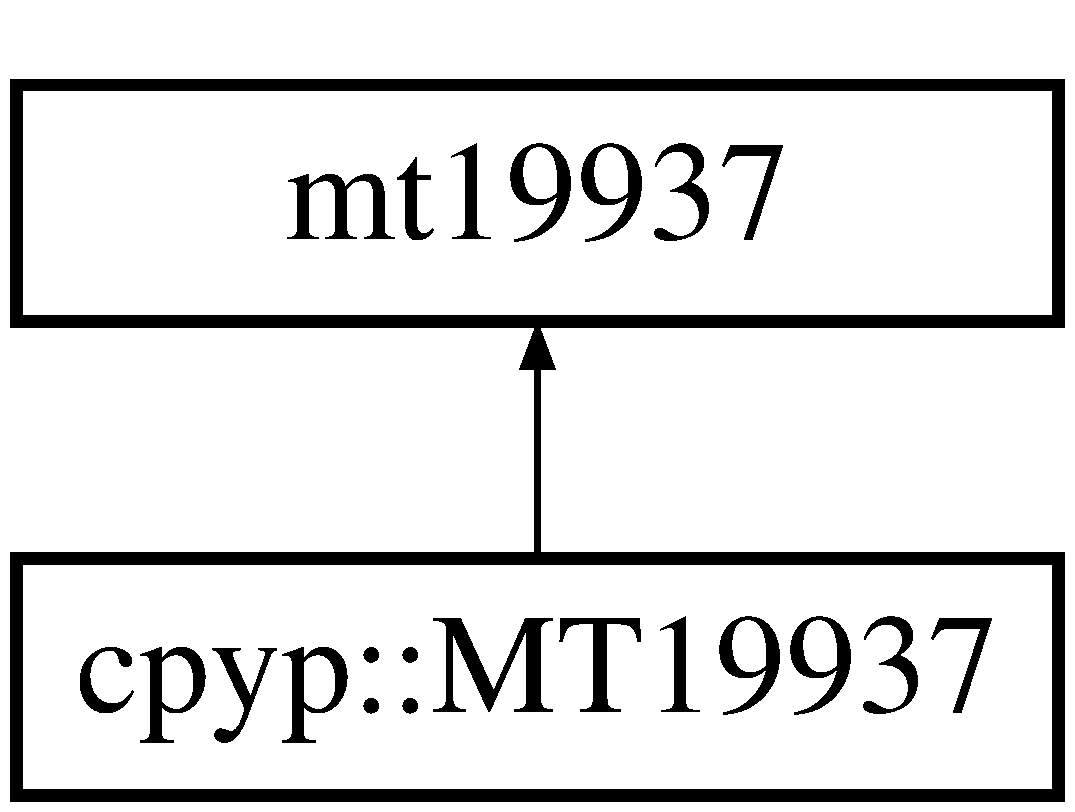
\includegraphics[height=2.000000cm]{structcpyp_1_1_m_t19937}
\end{center}
\end{figure}
\subsection*{Public Member Functions}
\begin{DoxyCompactItemize}
\item 
\mbox{\Hypertarget{structcpyp_1_1_m_t19937_aaaba5683758f3cdc63b2c35034aee5ed}\label{structcpyp_1_1_m_t19937_aaaba5683758f3cdc63b2c35034aee5ed}} 
{\bfseries M\+T19937} (uint32\+\_\+t s)
\end{DoxyCompactItemize}
\subsection*{Static Public Member Functions}
\begin{DoxyCompactItemize}
\item 
\mbox{\Hypertarget{structcpyp_1_1_m_t19937_a7f64402711c1e8c6d7ec0019414ac636}\label{structcpyp_1_1_m_t19937_a7f64402711c1e8c6d7ec0019414ac636}} 
static uint32\+\_\+t {\bfseries Get\+Truly\+Random\+Seed} ()
\end{DoxyCompactItemize}


The documentation for this struct was generated from the following file\+:\begin{DoxyCompactItemize}
\item 
random.\+h\end{DoxyCompactItemize}

\hypertarget{structcpyp_1_1multinomial__distribution}{}\section{cpyp\+:\+:multinomial\+\_\+distribution$<$ F $>$ Struct Template Reference}
\label{structcpyp_1_1multinomial__distribution}\index{cpyp\+::multinomial\+\_\+distribution$<$ F $>$@{cpyp\+::multinomial\+\_\+distribution$<$ F $>$}}
\subsection*{Public Member Functions}
\begin{DoxyCompactItemize}
\item 
\mbox{\Hypertarget{structcpyp_1_1multinomial__distribution_ab5853e699f1dbc23dddb36c63dd83888}\label{structcpyp_1_1multinomial__distribution_ab5853e699f1dbc23dddb36c63dd83888}} 
{\bfseries multinomial\+\_\+distribution} (const std\+::vector$<$ F $>$ \&v)
\item 
\mbox{\Hypertarget{structcpyp_1_1multinomial__distribution_aa1833522472255ef12889dfd6437c9cb}\label{structcpyp_1_1multinomial__distribution_aa1833522472255ef12889dfd6437c9cb}} 
{\footnotesize template$<$class Engine $>$ }\\unsigned {\bfseries operator()} (Engine \&eng) const
\end{DoxyCompactItemize}
\subsection*{Public Attributes}
\begin{DoxyCompactItemize}
\item 
\mbox{\Hypertarget{structcpyp_1_1multinomial__distribution_a65244e5dffdb1d4009e30fab7cd9894c}\label{structcpyp_1_1multinomial__distribution_a65244e5dffdb1d4009e30fab7cd9894c}} 
const std\+::vector$<$ F $>$ \& {\bfseries probs}
\item 
\mbox{\Hypertarget{structcpyp_1_1multinomial__distribution_a9f8fa8d7878356b92a4a36148f501216}\label{structcpyp_1_1multinomial__distribution_a9f8fa8d7878356b92a4a36148f501216}} 
const F {\bfseries sum}
\end{DoxyCompactItemize}


The documentation for this struct was generated from the following file\+:\begin{DoxyCompactItemize}
\item 
random.\+h\end{DoxyCompactItemize}

\hypertarget{structcpyp_1_1_pair_int_t}{}\section{cpyp\+:\+:Pair\+IntT$<$ T $>$ Struct Template Reference}
\label{structcpyp_1_1_pair_int_t}\index{cpyp\+::\+Pair\+Int\+T$<$ T $>$@{cpyp\+::\+Pair\+Int\+T$<$ T $>$}}
\subsection*{Public Member Functions}
\begin{DoxyCompactItemize}
\item 
\mbox{\Hypertarget{structcpyp_1_1_pair_int_t_a4e08e7614633c8c37f1a325e9b674356}\label{structcpyp_1_1_pair_int_t_a4e08e7614633c8c37f1a325e9b674356}} 
const \mbox{\hyperlink{structcpyp_1_1_pair_int_t}{Pair\+IntT}} \& {\bfseries operator=} (const std\+::pair$<$ const unsigned, T $>$ \&v)
\item 
\mbox{\Hypertarget{structcpyp_1_1_pair_int_t_a45cc2a19d5595d59efffff0aa848a548}\label{structcpyp_1_1_pair_int_t_a45cc2a19d5595d59efffff0aa848a548}} 
{\bfseries operator const std\+::pair$<$ const unsigned, T $>$ \&} () const
\item 
\mbox{\Hypertarget{structcpyp_1_1_pair_int_t_a32f82d1d08e5c4a69520dee4051c3792}\label{structcpyp_1_1_pair_int_t_a32f82d1d08e5c4a69520dee4051c3792}} 
unsigned \& {\bfseries first} ()
\item 
\mbox{\Hypertarget{structcpyp_1_1_pair_int_t_a32adb1aa9d8c8b2588ad3d52c3461e22}\label{structcpyp_1_1_pair_int_t_a32adb1aa9d8c8b2588ad3d52c3461e22}} 
T \& {\bfseries second} ()
\item 
\mbox{\Hypertarget{structcpyp_1_1_pair_int_t_a6229ee64da435cab964d1bed44404689}\label{structcpyp_1_1_pair_int_t_a6229ee64da435cab964d1bed44404689}} 
const unsigned \& {\bfseries first} () const
\item 
\mbox{\Hypertarget{structcpyp_1_1_pair_int_t_adf508769b7196ef9aac4c35a92350985}\label{structcpyp_1_1_pair_int_t_adf508769b7196ef9aac4c35a92350985}} 
const T \& {\bfseries second} () const
\end{DoxyCompactItemize}


The documentation for this struct was generated from the following file\+:\begin{DoxyCompactItemize}
\item 
msparse\+\_\+vector.\+h\end{DoxyCompactItemize}

\hypertarget{structcpyp_1_1_p_y_p_l_m}{}\section{cpyp\+:\+:P\+Y\+P\+LM$<$ N $>$ Struct Template Reference}
\label{structcpyp_1_1_p_y_p_l_m}\index{cpyp\+::\+P\+Y\+P\+L\+M$<$ N $>$@{cpyp\+::\+P\+Y\+P\+L\+M$<$ N $>$}}
\subsection*{Public Member Functions}
\begin{DoxyCompactItemize}
\item 
\mbox{\Hypertarget{structcpyp_1_1_p_y_p_l_m_af6ad8b19e6a37aa0abc885787e33e649}\label{structcpyp_1_1_p_y_p_l_m_af6ad8b19e6a37aa0abc885787e33e649}} 
{\bfseries P\+Y\+P\+LM} (unsigned vs, double da=1.\+0, double db=1.\+0, double ss=1.\+0, double sr=1.\+0)
\item 
\mbox{\Hypertarget{structcpyp_1_1_p_y_p_l_m_ab05d9800e3e62c87bb35bf5d8b4e3d67}\label{structcpyp_1_1_p_y_p_l_m_ab05d9800e3e62c87bb35bf5d8b4e3d67}} 
{\footnotesize template$<$typename Engine $>$ }\\void {\bfseries increment} (unsigned w, const std\+::vector$<$ unsigned $>$ \&context, Engine \&eng)
\item 
\mbox{\Hypertarget{structcpyp_1_1_p_y_p_l_m_af2a057a5d2d4ba6389e6fd9ef0756594}\label{structcpyp_1_1_p_y_p_l_m_af2a057a5d2d4ba6389e6fd9ef0756594}} 
{\footnotesize template$<$typename Engine $>$ }\\void {\bfseries decrement} (unsigned w, const std\+::vector$<$ unsigned $>$ \&context, Engine \&eng)
\item 
\mbox{\Hypertarget{structcpyp_1_1_p_y_p_l_m_ace332fabe9addb79cc5e68d6ab1884f5}\label{structcpyp_1_1_p_y_p_l_m_ace332fabe9addb79cc5e68d6ab1884f5}} 
double {\bfseries prob} (unsigned w, const std\+::vector$<$ unsigned $>$ \&context) const
\item 
\mbox{\Hypertarget{structcpyp_1_1_p_y_p_l_m_a1ce518c3aa817de05fd9259ba6e5b9da}\label{structcpyp_1_1_p_y_p_l_m_a1ce518c3aa817de05fd9259ba6e5b9da}} 
double {\bfseries log\+\_\+likelihood} () const
\item 
\mbox{\Hypertarget{structcpyp_1_1_p_y_p_l_m_a16776e9406d8a810cce71d9602aa139d}\label{structcpyp_1_1_p_y_p_l_m_a16776e9406d8a810cce71d9602aa139d}} 
{\footnotesize template$<$typename Engine $>$ }\\void {\bfseries resample\+\_\+hyperparameters} (Engine \&eng)
\item 
\mbox{\Hypertarget{structcpyp_1_1_p_y_p_l_m_a4fcee24f5150d8c4955f15e32f5992a0}\label{structcpyp_1_1_p_y_p_l_m_a4fcee24f5150d8c4955f15e32f5992a0}} 
{\footnotesize template$<$class Archive $>$ }\\void {\bfseries serialize} (Archive \&ar, const unsigned int version)
\item 
\mbox{\Hypertarget{structcpyp_1_1_p_y_p_l_m_a4543a079fb8612bd2dc8ec7e3e47ce1b}\label{structcpyp_1_1_p_y_p_l_m_a4543a079fb8612bd2dc8ec7e3e47ce1b}} 
void {\bfseries print} ()
\end{DoxyCompactItemize}
\subsection*{Public Attributes}
\begin{DoxyCompactItemize}
\item 
\mbox{\Hypertarget{structcpyp_1_1_p_y_p_l_m_abba5ef2af7b916ca595f3d9694c6a118}\label{structcpyp_1_1_p_y_p_l_m_abba5ef2af7b916ca595f3d9694c6a118}} 
\mbox{\hyperlink{structcpyp_1_1_p_y_p_l_m}{P\+Y\+P\+LM}}$<$ N-\/1 $>$ {\bfseries backoff}
\item 
\mbox{\Hypertarget{structcpyp_1_1_p_y_p_l_m_a8d438a19aadd12a046be958ffd0d5036}\label{structcpyp_1_1_p_y_p_l_m_a8d438a19aadd12a046be958ffd0d5036}} 
\mbox{\hyperlink{structcpyp_1_1tied__parameter__resampler}{tied\+\_\+parameter\+\_\+resampler}}$<$ \mbox{\hyperlink{classcpyp_1_1crp}{crp}}$<$ unsigned $>$ $>$ {\bfseries tr}
\item 
\mbox{\Hypertarget{structcpyp_1_1_p_y_p_l_m_a94340f4378e89d366c5c4db82d20f565}\label{structcpyp_1_1_p_y_p_l_m_a94340f4378e89d366c5c4db82d20f565}} 
std\+::vector$<$ unsigned $>$ {\bfseries lookup}
\item 
\mbox{\Hypertarget{structcpyp_1_1_p_y_p_l_m_aa9b766dc714a43aca4f109c53cacfeb2}\label{structcpyp_1_1_p_y_p_l_m_aa9b766dc714a43aca4f109c53cacfeb2}} 
std\+::unordered\+\_\+map$<$ std\+::vector$<$ unsigned $>$, \mbox{\hyperlink{classcpyp_1_1crp}{crp}}$<$ unsigned $>$, \mbox{\hyperlink{structuvector__hash}{uvector\+\_\+hash}} $>$ {\bfseries p}
\end{DoxyCompactItemize}


The documentation for this struct was generated from the following file\+:\begin{DoxyCompactItemize}
\item 
hpyplm.\+h\end{DoxyCompactItemize}

\hypertarget{structcpyp_1_1_p_y_p_l_m_3_010_01_4}{}\section{cpyp\+:\+:P\+Y\+P\+LM$<$ 0 $>$ Struct Template Reference}
\label{structcpyp_1_1_p_y_p_l_m_3_010_01_4}\index{cpyp\+::\+P\+Y\+P\+L\+M$<$ 0 $>$@{cpyp\+::\+P\+Y\+P\+L\+M$<$ 0 $>$}}
Inheritance diagram for cpyp\+:\+:P\+Y\+P\+LM$<$ 0 $>$\+:\begin{figure}[H]
\begin{center}
\leavevmode
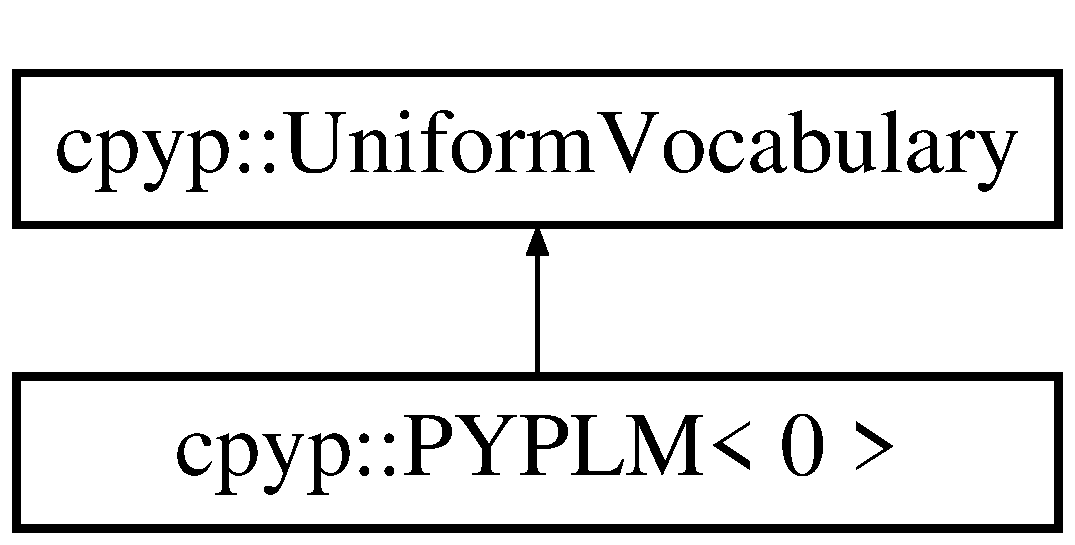
\includegraphics[height=2.000000cm]{structcpyp_1_1_p_y_p_l_m_3_010_01_4}
\end{center}
\end{figure}
\subsection*{Public Member Functions}
\begin{DoxyCompactItemize}
\item 
\mbox{\Hypertarget{structcpyp_1_1_p_y_p_l_m_3_010_01_4_ab145872943e246a33b1614e5fa86c56c}\label{structcpyp_1_1_p_y_p_l_m_3_010_01_4_ab145872943e246a33b1614e5fa86c56c}} 
{\bfseries P\+Y\+P\+LM} (unsigned vs, double a, double b, double c, double d)
\end{DoxyCompactItemize}
\subsection*{Additional Inherited Members}


The documentation for this struct was generated from the following file\+:\begin{DoxyCompactItemize}
\item 
hpyplm.\+h\end{DoxyCompactItemize}

\hypertarget{structcpyp_1_1slice__sampler__rfc__type}{}\section{cpyp\+:\+:slice\+\_\+sampler\+\_\+rfc\+\_\+type$<$ F, Fn, U $>$ Struct Template Reference}
\label{structcpyp_1_1slice__sampler__rfc__type}\index{cpyp\+::slice\+\_\+sampler\+\_\+rfc\+\_\+type$<$ F, Fn, U $>$@{cpyp\+::slice\+\_\+sampler\+\_\+rfc\+\_\+type$<$ F, Fn, U $>$}}


{\ttfamily \#include $<$slice\+\_\+sampler.\+h$>$}

\subsection*{Public Member Functions}
\begin{DoxyCompactItemize}
\item 
\mbox{\Hypertarget{structcpyp_1_1slice__sampler__rfc__type_a43fcfa551213dd6e02faf509bbd89e33}\label{structcpyp_1_1slice__sampler__rfc__type_a43fcfa551213dd6e02faf509bbd89e33}} 
{\bfseries slice\+\_\+sampler\+\_\+rfc\+\_\+type} (F min\+\_\+x, F max\+\_\+x, const Fn \&f, U max\+\_\+nfeval)
\item 
\mbox{\Hypertarget{structcpyp_1_1slice__sampler__rfc__type_abe2d56d33ffd7f5f3be0574d03d1476d}\label{structcpyp_1_1slice__sampler__rfc__type_abe2d56d33ffd7f5f3be0574d03d1476d}} 
F {\bfseries operator()} (F x)
\end{DoxyCompactItemize}
\subsection*{Public Attributes}
\begin{DoxyCompactItemize}
\item 
\mbox{\Hypertarget{structcpyp_1_1slice__sampler__rfc__type_a87dd40e39f8943d42d24b84e4cc9cbc8}\label{structcpyp_1_1slice__sampler__rfc__type_a87dd40e39f8943d42d24b84e4cc9cbc8}} 
F {\bfseries min\+\_\+x}
\item 
\mbox{\Hypertarget{structcpyp_1_1slice__sampler__rfc__type_a9d07fe96711633270344e3db812ea983}\label{structcpyp_1_1slice__sampler__rfc__type_a9d07fe96711633270344e3db812ea983}} 
F {\bfseries max\+\_\+x}
\item 
\mbox{\Hypertarget{structcpyp_1_1slice__sampler__rfc__type_a7a3ec759a7d29ad6789d40f758ad840c}\label{structcpyp_1_1slice__sampler__rfc__type_a7a3ec759a7d29ad6789d40f758ad840c}} 
const Fn \& {\bfseries f}
\item 
\mbox{\Hypertarget{structcpyp_1_1slice__sampler__rfc__type_aaaff851896cee8d50b09cca1fbd50a5a}\label{structcpyp_1_1slice__sampler__rfc__type_aaaff851896cee8d50b09cca1fbd50a5a}} 
U {\bfseries max\+\_\+nfeval}
\item 
\mbox{\Hypertarget{structcpyp_1_1slice__sampler__rfc__type_aee717877f7e0f43491a2396971c384c8}\label{structcpyp_1_1slice__sampler__rfc__type_aee717877f7e0f43491a2396971c384c8}} 
U {\bfseries nfeval}
\end{DoxyCompactItemize}


\subsection{Detailed Description}
\subsubsection*{template$<$typename F, typename Fn, typename U$>$\newline
struct cpyp\+::slice\+\_\+sampler\+\_\+rfc\+\_\+type$<$ F, Fn, U $>$}

\mbox{\hyperlink{structcpyp_1_1slice__sampler__rfc__type}{slice\+\_\+sampler\+\_\+rfc\+\_\+type}}\{\} returns the value of a user-\/specified function if the argument is within range, or -\/ infinity otherwise 

The documentation for this struct was generated from the following file\+:\begin{DoxyCompactItemize}
\item 
slice\+\_\+sampler.\+h\end{DoxyCompactItemize}

\hypertarget{classcpyp_1_1_sparse_vector}{}\section{cpyp\+:\+:Sparse\+Vector$<$ T, L\+O\+C\+A\+L\+\_\+\+M\+AX $>$ Class Template Reference}
\label{classcpyp_1_1_sparse_vector}\index{cpyp\+::\+Sparse\+Vector$<$ T, L\+O\+C\+A\+L\+\_\+\+M\+A\+X $>$@{cpyp\+::\+Sparse\+Vector$<$ T, L\+O\+C\+A\+L\+\_\+\+M\+A\+X $>$}}
\subsection*{Classes}
\begin{DoxyCompactItemize}
\item 
struct \mbox{\hyperlink{structcpyp_1_1_sparse_vector_1_1const__iterator}{const\+\_\+iterator}}
\item 
struct \mbox{\hyperlink{structcpyp_1_1_sparse_vector_1_1iterator}{iterator}}
\end{DoxyCompactItemize}
\subsection*{Public Member Functions}
\begin{DoxyCompactItemize}
\item 
\mbox{\Hypertarget{classcpyp_1_1_sparse_vector_a7fe9424c4508dee8a6bb7ef4aeb5cdff}\label{classcpyp_1_1_sparse_vector_a7fe9424c4508dee8a6bb7ef4aeb5cdff}} 
{\bfseries Sparse\+Vector} (const \mbox{\hyperlink{classcpyp_1_1_sparse_vector}{Sparse\+Vector}} \&other)
\item 
\mbox{\Hypertarget{classcpyp_1_1_sparse_vector_a7a82b07b1af74ad0b8c9dc406794b3ac}\label{classcpyp_1_1_sparse_vector_a7a82b07b1af74ad0b8c9dc406794b3ac}} 
{\bfseries Sparse\+Vector} (std\+::pair$<$ unsigned, T $>$ $\ast$first, std\+::pair$<$ unsigned, T $>$ $\ast$last)
\item 
\mbox{\Hypertarget{classcpyp_1_1_sparse_vector_a28b325943fc12feb4b36356c2fa9b473}\label{classcpyp_1_1_sparse_vector_a28b325943fc12feb4b36356c2fa9b473}} 
void {\bfseries erase} (unsigned k)
\item 
\mbox{\Hypertarget{classcpyp_1_1_sparse_vector_aa1b26f2ae6f7d21b9e608a400ab937f2}\label{classcpyp_1_1_sparse_vector_aa1b26f2ae6f7d21b9e608a400ab937f2}} 
const \mbox{\hyperlink{classcpyp_1_1_sparse_vector}{Sparse\+Vector}}$<$ T $>$ \& {\bfseries operator=} (const \mbox{\hyperlink{classcpyp_1_1_sparse_vector}{Sparse\+Vector}}$<$ T $>$ \&other)
\item 
\mbox{\Hypertarget{classcpyp_1_1_sparse_vector_a59c60662068e05f96d2e14203b5b809f}\label{classcpyp_1_1_sparse_vector_a59c60662068e05f96d2e14203b5b809f}} 
T const  \& {\bfseries get\+\_\+singleton} () const
\item 
\mbox{\Hypertarget{classcpyp_1_1_sparse_vector_a5e399e98e6f431bc95b315edea3de475}\label{classcpyp_1_1_sparse_vector_a5e399e98e6f431bc95b315edea3de475}} 
bool {\bfseries nonzero} (unsigned k) const
\item 
\mbox{\Hypertarget{classcpyp_1_1_sparse_vector_aadc7ed9b0ad723ceccae00fe5514df06}\label{classcpyp_1_1_sparse_vector_aadc7ed9b0ad723ceccae00fe5514df06}} 
T \& {\bfseries operator\mbox{[}$\,$\mbox{]}} (unsigned k)
\item 
\mbox{\Hypertarget{classcpyp_1_1_sparse_vector_aaa2a8471f5fd47adb22ee5910fe7f9b8}\label{classcpyp_1_1_sparse_vector_aaa2a8471f5fd47adb22ee5910fe7f9b8}} 
void {\bfseries set\+\_\+value} (unsigned k, const T \&v)
\item 
\mbox{\Hypertarget{classcpyp_1_1_sparse_vector_a3d9440aedabf41acd21e20504fa310c5}\label{classcpyp_1_1_sparse_vector_a3d9440aedabf41acd21e20504fa310c5}} 
T \& {\bfseries add\+\_\+value} (unsigned k, const T \&v)
\item 
\mbox{\Hypertarget{classcpyp_1_1_sparse_vector_a6ff198d4f5e1bde25f3a9aaba13c094e}\label{classcpyp_1_1_sparse_vector_a6ff198d4f5e1bde25f3a9aaba13c094e}} 
T {\bfseries get} (unsigned k) const
\item 
\mbox{\Hypertarget{classcpyp_1_1_sparse_vector_a60728a19fc2b207979c1bd0a1b63b611}\label{classcpyp_1_1_sparse_vector_a60728a19fc2b207979c1bd0a1b63b611}} 
T {\bfseries value} (unsigned k) const
\item 
\mbox{\Hypertarget{classcpyp_1_1_sparse_vector_a22be6f6912f469706cf2f798201a6a9e}\label{classcpyp_1_1_sparse_vector_a22be6f6912f469706cf2f798201a6a9e}} 
T {\bfseries l2norm\+\_\+sq} () const
\item 
\mbox{\Hypertarget{classcpyp_1_1_sparse_vector_a06285bc0fcf3dd86664aef6415269d42}\label{classcpyp_1_1_sparse_vector_a06285bc0fcf3dd86664aef6415269d42}} 
T {\bfseries l2norm} () const
\item 
\mbox{\Hypertarget{classcpyp_1_1_sparse_vector_a95d0a840d1eb71705c17ff22bd498257}\label{classcpyp_1_1_sparse_vector_a95d0a840d1eb71705c17ff22bd498257}} 
T {\bfseries pnorm} (const double p) const
\item 
\mbox{\Hypertarget{classcpyp_1_1_sparse_vector_a8232c9fda49960e650478c9c9de8b416}\label{classcpyp_1_1_sparse_vector_a8232c9fda49960e650478c9c9de8b416}} 
{\footnotesize template$<$typename S $>$ }\\S {\bfseries tanimoto\+\_\+coef} (const \mbox{\hyperlink{classcpyp_1_1_sparse_vector}{Sparse\+Vector}}$<$ S $>$ \&vec) const
\item 
\mbox{\Hypertarget{classcpyp_1_1_sparse_vector_a45922a4c5be95d6e72c119c15bf8c404}\label{classcpyp_1_1_sparse_vector_a45922a4c5be95d6e72c119c15bf8c404}} 
size\+\_\+t {\bfseries size} () const
\item 
\mbox{\Hypertarget{classcpyp_1_1_sparse_vector_a5f8f3b62adebeece48b0dec6a9cb1bf8}\label{classcpyp_1_1_sparse_vector_a5f8f3b62adebeece48b0dec6a9cb1bf8}} 
size\+\_\+t {\bfseries num\+\_\+nonzero} () const
\item 
\mbox{\Hypertarget{classcpyp_1_1_sparse_vector_ae11acd5c8f6fcea5cb98262d674a5711}\label{classcpyp_1_1_sparse_vector_ae11acd5c8f6fcea5cb98262d674a5711}} 
void {\bfseries clear} ()
\item 
\mbox{\Hypertarget{classcpyp_1_1_sparse_vector_ab6b5047179057f594120784fe54eebdd}\label{classcpyp_1_1_sparse_vector_ab6b5047179057f594120784fe54eebdd}} 
bool {\bfseries empty} () const
\item 
\mbox{\Hypertarget{classcpyp_1_1_sparse_vector_a060ea06d6b5426e06947931b0a05ae6c}\label{classcpyp_1_1_sparse_vector_a060ea06d6b5426e06947931b0a05ae6c}} 
\mbox{\hyperlink{classcpyp_1_1_sparse_vector}{Sparse\+Vector}} \& {\bfseries operator+=} (const \mbox{\hyperlink{classcpyp_1_1_sparse_vector}{Sparse\+Vector}} \&other)
\item 
\mbox{\Hypertarget{classcpyp_1_1_sparse_vector_a56b0f9bcfacc501b49fd4fdb0f50c44c}\label{classcpyp_1_1_sparse_vector_a56b0f9bcfacc501b49fd4fdb0f50c44c}} 
{\footnotesize template$<$typename O $>$ }\\\mbox{\hyperlink{classcpyp_1_1_sparse_vector}{Sparse\+Vector}} \& {\bfseries operator+=} (const \mbox{\hyperlink{classcpyp_1_1_sparse_vector}{Sparse\+Vector}}$<$ O $>$ \&other)
\item 
\mbox{\Hypertarget{classcpyp_1_1_sparse_vector_a49594df40000b3985af19df84007f15f}\label{classcpyp_1_1_sparse_vector_a49594df40000b3985af19df84007f15f}} 
{\footnotesize template$<$typename O $>$ }\\void {\bfseries plus\+\_\+eq\+\_\+v\+\_\+times\+\_\+s} (const \mbox{\hyperlink{classcpyp_1_1_sparse_vector}{Sparse\+Vector}}$<$ O $>$ \&other, const O scalar)
\item 
\mbox{\Hypertarget{classcpyp_1_1_sparse_vector_a68b75ee85385070d85657219b358ca7b}\label{classcpyp_1_1_sparse_vector_a68b75ee85385070d85657219b358ca7b}} 
\mbox{\hyperlink{classcpyp_1_1_sparse_vector}{Sparse\+Vector}} \& {\bfseries operator-\/=} (const \mbox{\hyperlink{classcpyp_1_1_sparse_vector}{Sparse\+Vector}} \&other)
\item 
\mbox{\Hypertarget{classcpyp_1_1_sparse_vector_a402c045bd9b8126a35f865a76870e1c6}\label{classcpyp_1_1_sparse_vector_a402c045bd9b8126a35f865a76870e1c6}} 
\mbox{\hyperlink{classcpyp_1_1_sparse_vector}{Sparse\+Vector}} \& {\bfseries operator$\ast$=} (const T \&scalar)
\item 
\mbox{\Hypertarget{classcpyp_1_1_sparse_vector_a3bec2d66757d348ea72bbd16d3afe90a}\label{classcpyp_1_1_sparse_vector_a3bec2d66757d348ea72bbd16d3afe90a}} 
\mbox{\hyperlink{classcpyp_1_1_sparse_vector}{Sparse\+Vector}} \& {\bfseries operator/=} (const T \&scalar)
\item 
\mbox{\Hypertarget{classcpyp_1_1_sparse_vector_acc496c92f53002a95fec694ee9d5fcc6}\label{classcpyp_1_1_sparse_vector_acc496c92f53002a95fec694ee9d5fcc6}} 
\mbox{\hyperlink{classcpyp_1_1_sparse_vector}{Sparse\+Vector}}$<$ T $>$ {\bfseries erase\+\_\+zeros} (const T \&E\+P\+S\+I\+L\+ON=1e-\/4) const
\item 
\mbox{\Hypertarget{classcpyp_1_1_sparse_vector_a34bf71e6275b54c7608508a5c251dc37}\label{classcpyp_1_1_sparse_vector_a34bf71e6275b54c7608508a5c251dc37}} 
\mbox{\hyperlink{structcpyp_1_1_sparse_vector_1_1iterator}{iterator}} {\bfseries find} (unsigned k)
\item 
\mbox{\Hypertarget{classcpyp_1_1_sparse_vector_a21773e7e8128c0f17b062795c9ebe239}\label{classcpyp_1_1_sparse_vector_a21773e7e8128c0f17b062795c9ebe239}} 
\mbox{\hyperlink{structcpyp_1_1_sparse_vector_1_1iterator}{iterator}} {\bfseries begin} ()
\item 
\mbox{\Hypertarget{classcpyp_1_1_sparse_vector_ab5cd903c798c3f649fd9471f7369ccd3}\label{classcpyp_1_1_sparse_vector_ab5cd903c798c3f649fd9471f7369ccd3}} 
\mbox{\hyperlink{structcpyp_1_1_sparse_vector_1_1iterator}{iterator}} {\bfseries end} ()
\item 
\mbox{\Hypertarget{classcpyp_1_1_sparse_vector_acacf23282cdeaa77a2b2c9dddd9a8327}\label{classcpyp_1_1_sparse_vector_acacf23282cdeaa77a2b2c9dddd9a8327}} 
\mbox{\hyperlink{structcpyp_1_1_sparse_vector_1_1const__iterator}{const\+\_\+iterator}} {\bfseries find} (unsigned k) const
\item 
\mbox{\Hypertarget{classcpyp_1_1_sparse_vector_a7fc6f661fefc739871b7718cfa70f9b1}\label{classcpyp_1_1_sparse_vector_a7fc6f661fefc739871b7718cfa70f9b1}} 
\mbox{\hyperlink{structcpyp_1_1_sparse_vector_1_1const__iterator}{const\+\_\+iterator}} {\bfseries begin} () const
\item 
\mbox{\Hypertarget{classcpyp_1_1_sparse_vector_a425e531a0ef32ceec8772072ad107524}\label{classcpyp_1_1_sparse_vector_a425e531a0ef32ceec8772072ad107524}} 
\mbox{\hyperlink{structcpyp_1_1_sparse_vector_1_1const__iterator}{const\+\_\+iterator}} {\bfseries end} () const
\item 
\mbox{\Hypertarget{classcpyp_1_1_sparse_vector_a53eb971c2d78befb5d9eef9afc55488b}\label{classcpyp_1_1_sparse_vector_a53eb971c2d78befb5d9eef9afc55488b}} 
void {\bfseries init\+\_\+vector} (std\+::vector$<$ T $>$ $\ast$vp) const
\item 
\mbox{\Hypertarget{classcpyp_1_1_sparse_vector_abfe6a0368faac0dfd883e96e27d228d6}\label{classcpyp_1_1_sparse_vector_abfe6a0368faac0dfd883e96e27d228d6}} 
void {\bfseries init\+\_\+vector} (std\+::vector$<$ T $>$ \&v) const
\item 
\mbox{\Hypertarget{classcpyp_1_1_sparse_vector_a8edef03778570d73e923fc65b4c3cb4b}\label{classcpyp_1_1_sparse_vector_a8edef03778570d73e923fc65b4c3cb4b}} 
T {\bfseries dot} (const std\+::vector$<$ T $>$ \&v) const
\item 
\mbox{\Hypertarget{classcpyp_1_1_sparse_vector_a90c9d4bca95c9bc4a5ee406800fc124b}\label{classcpyp_1_1_sparse_vector_a90c9d4bca95c9bc4a5ee406800fc124b}} 
T {\bfseries dot} (const \mbox{\hyperlink{classcpyp_1_1_sparse_vector}{Sparse\+Vector}}$<$ T $>$ \&other) const
\item 
\mbox{\Hypertarget{classcpyp_1_1_sparse_vector_ac35c07d95026e5585a056402b5f44739}\label{classcpyp_1_1_sparse_vector_ac35c07d95026e5585a056402b5f44739}} 
bool {\bfseries operator==} (const \mbox{\hyperlink{classcpyp_1_1_sparse_vector}{Sparse\+Vector}}$<$ T $>$ \&other) const
\item 
\mbox{\Hypertarget{classcpyp_1_1_sparse_vector_ab48e4e466ac30efb7859f5f5c1bffb1b}\label{classcpyp_1_1_sparse_vector_ab48e4e466ac30efb7859f5f5c1bffb1b}} 
void {\bfseries swap} (\mbox{\hyperlink{classcpyp_1_1_sparse_vector}{Sparse\+Vector}}$<$ T $>$ \&other)
\item 
\mbox{\Hypertarget{classcpyp_1_1_sparse_vector_a70497bd7e6b62ebf678fec01c394138f}\label{classcpyp_1_1_sparse_vector_a70497bd7e6b62ebf678fec01c394138f}} 
{\footnotesize template$<$class Archive $>$ }\\void {\bfseries save} (Archive \&ar, const unsigned int) const
\item 
\mbox{\Hypertarget{classcpyp_1_1_sparse_vector_aec6d230f8d1bc68f17015623aafb6244}\label{classcpyp_1_1_sparse_vector_aec6d230f8d1bc68f17015623aafb6244}} 
{\footnotesize template$<$class Archive $>$ }\\void {\bfseries load} (Archive \&ar, const unsigned int)
\end{DoxyCompactItemize}


The documentation for this class was generated from the following file\+:\begin{DoxyCompactItemize}
\item 
msparse\+\_\+vector.\+h\end{DoxyCompactItemize}

\hypertarget{classcpyp_1_1_s_p_y_p_l_m}{}\section{cpyp\+:\+:S\+P\+Y\+P\+LM$<$ N $>$ Class Template Reference}
\label{classcpyp_1_1_s_p_y_p_l_m}\index{cpyp\+::\+S\+P\+Y\+P\+L\+M$<$ N $>$@{cpyp\+::\+S\+P\+Y\+P\+L\+M$<$ N $>$}}
\subsection*{Public Member Functions}
\begin{DoxyCompactItemize}
\item 
\mbox{\Hypertarget{classcpyp_1_1_s_p_y_p_l_m_a33f27e864901666766ab1355314aa9e2}\label{classcpyp_1_1_s_p_y_p_l_m_a33f27e864901666766ab1355314aa9e2}} 
{\bfseries S\+P\+Y\+P\+LM} (unsigned vs, unsigned n\+\_\+txt, std\+::vector$<$ unsigned $>$ num\+\_\+of\+\_\+words\+\_\+per\+\_\+text, double da=1.\+0, double db=1.\+0, double ss=1.\+0, double sr=1.\+0, double lambda=0.\+5, double a\+\_\+in=1.\+0, double b\+\_\+in=1.\+0)
\item 
\mbox{\Hypertarget{classcpyp_1_1_s_p_y_p_l_m_a411e0a1221c00b3c68bcc6e577057932}\label{classcpyp_1_1_s_p_y_p_l_m_a411e0a1221c00b3c68bcc6e577057932}} 
{\footnotesize template$<$typename Engine $>$ }\\void {\bfseries increment} (unsigned w, const std\+::vector$<$ unsigned $>$ \&context, unsigned int j, unsigned int \&r, Engine \&eng)
\item 
\mbox{\Hypertarget{classcpyp_1_1_s_p_y_p_l_m_ab0c6563b5c5c36e4627f1d50bc796550}\label{classcpyp_1_1_s_p_y_p_l_m_ab0c6563b5c5c36e4627f1d50bc796550}} 
{\footnotesize template$<$typename Engine $>$ }\\void {\bfseries decrement} (unsigned w, const std\+::vector$<$ unsigned $>$ \&context, unsigned j, bool r, Engine \&eng)
\item 
\mbox{\Hypertarget{classcpyp_1_1_s_p_y_p_l_m_a06e8add5ae77abc876e47c57027c47e2}\label{classcpyp_1_1_s_p_y_p_l_m_a06e8add5ae77abc876e47c57027c47e2}} 
{\footnotesize template$<$typename Engine $>$ }\\void {\bfseries resample\+\_\+hyperparameters} (Engine \&eng)
\item 
\mbox{\Hypertarget{classcpyp_1_1_s_p_y_p_l_m_a89d75da65191519bb0be78bea318eb3e}\label{classcpyp_1_1_s_p_y_p_l_m_a89d75da65191519bb0be78bea318eb3e}} 
{\footnotesize template$<$typename Engine $>$ }\\void {\bfseries resample\+\_\+lambda\+\_\+parameters} (Engine \&eng)
\item 
\mbox{\Hypertarget{classcpyp_1_1_s_p_y_p_l_m_abf4ffcf23da3b5ade1fc70351099b15e}\label{classcpyp_1_1_s_p_y_p_l_m_abf4ffcf23da3b5ade1fc70351099b15e}} 
double {\bfseries logsumexp} (std\+::vector$<$ double $>$ \&nums)
\item 
\mbox{\Hypertarget{classcpyp_1_1_s_p_y_p_l_m_ad6c2cd1b003d6e655449c28308d5d830}\label{classcpyp_1_1_s_p_y_p_l_m_ad6c2cd1b003d6e655449c28308d5d830}} 
double {\bfseries prob} (unsigned w, const std\+::vector$<$ unsigned $>$ \&context, const unsigned j) const
\item 
\mbox{\Hypertarget{classcpyp_1_1_s_p_y_p_l_m_aba3967b8514bb07eced3ee2977916cb4}\label{classcpyp_1_1_s_p_y_p_l_m_aba3967b8514bb07eced3ee2977916cb4}} 
double {\bfseries log\+\_\+likelihood} (const unsigned j)
\item 
\mbox{\Hypertarget{classcpyp_1_1_s_p_y_p_l_m_a85178a9a55b701b64d62acb74527fc87}\label{classcpyp_1_1_s_p_y_p_l_m_a85178a9a55b701b64d62acb74527fc87}} 
void {\bfseries print} ()
\end{DoxyCompactItemize}


The documentation for this class was generated from the following file\+:\begin{DoxyCompactItemize}
\item 
shpyplm.\+h\end{DoxyCompactItemize}

\hypertarget{structcpyp_1_1tied__parameter__resampler}{}\section{cpyp\+:\+:tied\+\_\+parameter\+\_\+resampler$<$ C\+RP $>$ Struct Template Reference}
\label{structcpyp_1_1tied__parameter__resampler}\index{cpyp\+::tied\+\_\+parameter\+\_\+resampler$<$ C\+R\+P $>$@{cpyp\+::tied\+\_\+parameter\+\_\+resampler$<$ C\+R\+P $>$}}
\subsection*{Public Member Functions}
\begin{DoxyCompactItemize}
\item 
\mbox{\Hypertarget{structcpyp_1_1tied__parameter__resampler_a4946bd4b8ffd32347a60145784c4f68f}\label{structcpyp_1_1tied__parameter__resampler_a4946bd4b8ffd32347a60145784c4f68f}} 
{\bfseries tied\+\_\+parameter\+\_\+resampler} (double da, double db, double ss, double sr, double d=0.\+5, double s=1.\+0)
\item 
\mbox{\Hypertarget{structcpyp_1_1tied__parameter__resampler_abdbfcf9c749de11c2c9c5e142eb95b68}\label{structcpyp_1_1tied__parameter__resampler_abdbfcf9c749de11c2c9c5e142eb95b68}} 
void {\bfseries insert} (C\+RP $\ast$\mbox{\hyperlink{classcpyp_1_1crp}{crp}})
\item 
\mbox{\Hypertarget{structcpyp_1_1tied__parameter__resampler_a6cff17a9e2b41cda54d8c981d29230de}\label{structcpyp_1_1tied__parameter__resampler_a6cff17a9e2b41cda54d8c981d29230de}} 
void {\bfseries erase} (C\+RP $\ast$\mbox{\hyperlink{classcpyp_1_1crp}{crp}})
\item 
\mbox{\Hypertarget{structcpyp_1_1tied__parameter__resampler_a1432fb2c27862e1ace80bc0dd83c158c}\label{structcpyp_1_1tied__parameter__resampler_a1432fb2c27862e1ace80bc0dd83c158c}} 
size\+\_\+t {\bfseries size} () const
\item 
\mbox{\Hypertarget{structcpyp_1_1tied__parameter__resampler_a60f2775d17a18cad08683ebf8072fdfd}\label{structcpyp_1_1tied__parameter__resampler_a60f2775d17a18cad08683ebf8072fdfd}} 
double {\bfseries log\+\_\+likelihood} (double d, double s) const
\item 
\mbox{\Hypertarget{structcpyp_1_1tied__parameter__resampler_ad0e9ac79b178e48f27f92ad36089aba5}\label{structcpyp_1_1tied__parameter__resampler_ad0e9ac79b178e48f27f92ad36089aba5}} 
double {\bfseries log\+\_\+likelihood} () const
\item 
\mbox{\Hypertarget{structcpyp_1_1tied__parameter__resampler_a540c37cb69e75063c842aa70c653007b}\label{structcpyp_1_1tied__parameter__resampler_a540c37cb69e75063c842aa70c653007b}} 
{\footnotesize template$<$typename Engine $>$ }\\void {\bfseries resample\+\_\+hyperparameters} (Engine \&eng, const unsigned nloop=5, const unsigned niterations=10)
\end{DoxyCompactItemize}


The documentation for this struct was generated from the following file\+:\begin{DoxyCompactItemize}
\item 
tied\+\_\+parameter\+\_\+resampler.\+h\end{DoxyCompactItemize}

\hypertarget{structcpyp_1_1_uniform_vocabulary}{}\section{cpyp\+:\+:Uniform\+Vocabulary Struct Reference}
\label{structcpyp_1_1_uniform_vocabulary}\index{cpyp\+::\+Uniform\+Vocabulary@{cpyp\+::\+Uniform\+Vocabulary}}
Inheritance diagram for cpyp\+:\+:Uniform\+Vocabulary\+:\begin{figure}[H]
\begin{center}
\leavevmode
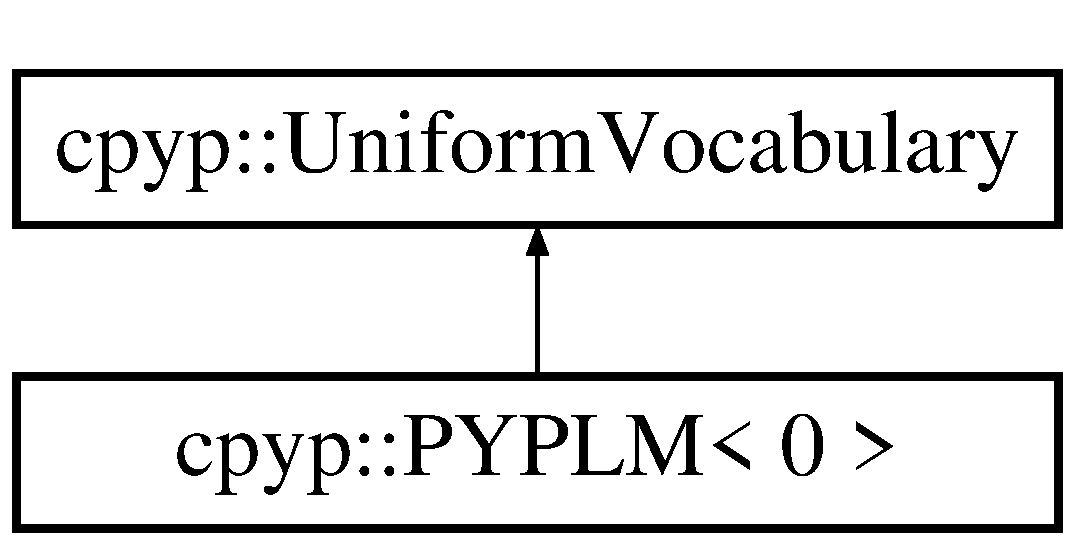
\includegraphics[height=2.000000cm]{structcpyp_1_1_uniform_vocabulary}
\end{center}
\end{figure}
\subsection*{Public Member Functions}
\begin{DoxyCompactItemize}
\item 
\mbox{\Hypertarget{structcpyp_1_1_uniform_vocabulary_a9f7977faa77d41408c8cf18b61bb6311}\label{structcpyp_1_1_uniform_vocabulary_a9f7977faa77d41408c8cf18b61bb6311}} 
{\bfseries Uniform\+Vocabulary} (unsigned vs, double, double, double, double)
\item 
\mbox{\Hypertarget{structcpyp_1_1_uniform_vocabulary_af6fe1630beb086b0e4d5ab894f49b6c0}\label{structcpyp_1_1_uniform_vocabulary_af6fe1630beb086b0e4d5ab894f49b6c0}} 
{\footnotesize template$<$typename Engine $>$ }\\void {\bfseries increment} (unsigned, const std\+::vector$<$ unsigned $>$ \&, Engine \&)
\item 
\mbox{\Hypertarget{structcpyp_1_1_uniform_vocabulary_a7295a1b3487dc4ed6c8349f5d1bdcd80}\label{structcpyp_1_1_uniform_vocabulary_a7295a1b3487dc4ed6c8349f5d1bdcd80}} 
{\footnotesize template$<$typename Engine $>$ }\\void {\bfseries decrement} (unsigned, const std\+::vector$<$ unsigned $>$ \&, Engine \&)
\item 
\mbox{\Hypertarget{structcpyp_1_1_uniform_vocabulary_af741559cf29e6ce5e60176c0ca5c6647}\label{structcpyp_1_1_uniform_vocabulary_af741559cf29e6ce5e60176c0ca5c6647}} 
double {\bfseries prob} (unsigned, const std\+::vector$<$ unsigned $>$ \&) const
\item 
\mbox{\Hypertarget{structcpyp_1_1_uniform_vocabulary_ab65db811af65ef52f5e6fbe36f0d70ef}\label{structcpyp_1_1_uniform_vocabulary_ab65db811af65ef52f5e6fbe36f0d70ef}} 
{\footnotesize template$<$typename Engine $>$ }\\void {\bfseries resample\+\_\+hyperparameters} (Engine \&)
\item 
\mbox{\Hypertarget{structcpyp_1_1_uniform_vocabulary_a690aa3198213c4984043baf9ed07bb4e}\label{structcpyp_1_1_uniform_vocabulary_a690aa3198213c4984043baf9ed07bb4e}} 
double {\bfseries log\+\_\+likelihood} () const
\item 
\mbox{\Hypertarget{structcpyp_1_1_uniform_vocabulary_ab7d2652fe8444150a332e3a2c0b77231}\label{structcpyp_1_1_uniform_vocabulary_ab7d2652fe8444150a332e3a2c0b77231}} 
{\footnotesize template$<$class Archive $>$ }\\void {\bfseries serialize} (Archive \&ar, const unsigned int)
\end{DoxyCompactItemize}
\subsection*{Public Attributes}
\begin{DoxyCompactItemize}
\item 
\mbox{\Hypertarget{structcpyp_1_1_uniform_vocabulary_a17aa628296af1f0f79bc5fb53b13ab5a}\label{structcpyp_1_1_uniform_vocabulary_a17aa628296af1f0f79bc5fb53b13ab5a}} 
double {\bfseries p0}
\item 
\mbox{\Hypertarget{structcpyp_1_1_uniform_vocabulary_a24c863368834ca1b1bcb8a39983501db}\label{structcpyp_1_1_uniform_vocabulary_a24c863368834ca1b1bcb8a39983501db}} 
int {\bfseries draws}
\end{DoxyCompactItemize}


The documentation for this struct was generated from the following file\+:\begin{DoxyCompactItemize}
\item 
uniform\+\_\+vocab.\+h\end{DoxyCompactItemize}

\hypertarget{structuvector__hash}{}\section{uvector\+\_\+hash Struct Reference}
\label{structuvector__hash}\index{uvector\+\_\+hash@{uvector\+\_\+hash}}
\subsection*{Public Member Functions}
\begin{DoxyCompactItemize}
\item 
\mbox{\Hypertarget{structuvector__hash_a73e5b313f892d888f72b82ef9e2f7bbf}\label{structuvector__hash_a73e5b313f892d888f72b82ef9e2f7bbf}} 
size\+\_\+t {\bfseries operator()} (const std\+::vector$<$ unsigned $>$ \&v) const
\end{DoxyCompactItemize}


The documentation for this struct was generated from the following file\+:\begin{DoxyCompactItemize}
\item 
uvector.\+h\end{DoxyCompactItemize}

%--- End generated contents ---

% Index
\backmatter
\newpage
\phantomsection
\clearemptydoublepage
\addcontentsline{toc}{chapter}{\indexname}
\printindex

\end{document}
